%
% File tto2019.tex
%
%% Based on the style files for ACL 2019, ACL 2018, NAACL 2018/19, which were
%% Based on the style files for ACL-2015, with some improvements
%%  taken from the NAACL-2016 style
%% Based on the style files for ACL-2014, which were, in turn,
%% based on ACL-2013, ACL-2012, ACL-2011, ACL-2010, ACL-IJCNLP-2009,
%% EACL-2009, IJCNLP-2008...
%% Based on the style files for EACL 2006 by 
%%e.agirre@ehu.es or Sergi.Balari@uab.es
%% and that of ACL 08 by Joakim Nivre and Noah Smith

\documentclass[11pt,a4paper]{article}
\usepackage[hyperref]{tto2019}
\usepackage{times}
\usepackage{latexsym}
\usepackage{multicol}
\usepackage{graphicx}

\usepackage{url}

%\aclfinalcopy % Uncomment this line for the final submission

%\setlength\titlebox{5cm}
% You can expand the titlebox if you need extra space
% to show all the authors. Please do not make the titlebox
% smaller than 5cm (the original size); we will check this
% in the camera-ready version and ask you to change it back.

\newcommand\BibTeX{B\textsc{ib}\TeX}

\title{Instructions for TTO 2019 Proceedings}

\author{First Author \\
  Affiliation / Address line 1 \\
  Affiliation / Address line 2 \\
  Affiliation / Address line 3 \\
  \texttt{email@domain} \\\And
  Second Author \\
  Affiliation / Address line 1 \\
  Affiliation / Address line 2 \\
  Affiliation / Address line 3 \\
  \texttt{email@domain} \\}

\date{}

\begin{document}
\maketitle
\begin{abstract}

\end{abstract}

\section{Introduction}


A number of recent studies  point towards the idea that ``Fake News'' or disinformation is a small subset of the total supply of information on online social networking platforms (e.g. Grinberg et al. (2019)~\cite{grinberg} and Broniatowski et al. (2020)~\cite{broniatowski}). Yet, this seemingly small subset is generating great concern in traditional media and in society in a broader sense. 

Section $230$ in the United States Communications Decency Act\footnote{Similar regulation exists in the European Union, see articles $12$ and $15$ of the E-commerce Directive (2000). } provides immunity for website platforms against the content created by users. Nevertheless, there is growing pressure for Mainstream Social Media Platforms (hereafter MSMP), such as Facebook, Twitter or Youtube, to moderate the available content. In particular, platforms seem to take explicit actions when content is in violation of local laws in different jurisdictions, e.g. laws regarding defamation of a racial nature, dissemination of symbols from unconstitutional organizations, privacy protection, digital security, electoral laws. Facebook reports having implemented a total of $64.7$ thousand content restrictions based on local law across all countries in 2020.\footnote{See Facebook Transparency Center, Content restrictions based on Local Law: \href{https://transparency.fb.com/data/content\-restrictions}{https://transparency.fb.com/data/content\-restrictions}. We summed the count of content restrictions over all countries reported in the table, for $H1$ and $H2$ of the year 2020.} Google reports a total of $26$ thousand government requests to remove content from July 2020 to December 2020, among which $11.4$ thousand concerned Youtube.\footnote{See Google's Transparency report, government requests to remove content: \href{https://transparencyreport.google.com/government-removals/overview}{https://transparencyreport.google.com/government-removals/overview}.} Twitter reports having received $42.2$ thousand legal demands from third-parties from January to June 2020, and has responded by withholding $82$ thousand accounts and $3.1$ thousand tweets.\footnote{See Twitter Transparency website, Removal requests: \href{https://transparency.twitter.com/en/reports/removal-requests.html\#2020-jan-jun}{https://transparency.twitter.com/en/reports/removal-requests.html\#2020-jan-jun}.} 

\smallskip

Furthermore, MSMP are increasingly engaging in editorial tasks by implementing targeted policies to insure that each platform's rules are not violated. Community guidelines of Facebook, Twitter and Youtube can be summarized in a handful of categories, regarding safety, privacy and authenticity; which include violence, terrorism, child sexual exploitation, abuse, harassment, hateful conduct, suicide or self-harm, illegal or regulated goods and services, platform manipulation and spam.\footnote{For an exhaustive overview of the community guidelines of Facebook, see: \href{https://www.facebook.com/communitystandards/}{https://www.facebook.com/communitystandards/}, for Twitter see: \href{https://help.twitter.com/en/rules-and-policies/twitter-rules}{https://help.twitter.com/en/rules-and-policies/twitter-rules}, and for Youtube see: \href{https://www.youtube.com/intl/en\_us/howyoutubeworks/policies/community\-guidelines/}{https://www.youtube.com/intl/en\_us/howyoutubeworks/policies/community\-guidelines/}.} While specific to each platform, the previously cited categories correspond in most cases to well defined concepts that fall into legal frameworks in many countries. In this article, we focus on MSMP's policies and actions regarding content with low credibility or false information, commonly referred to as {\it Fake News}.\footnote{For an overview on the {\it concept} of {\it Fake News}, we refer the reader to the article The science of fake news by Lazer et al. (2018)~\cite{lazer}.} The {\it Fake News} phenomenon is still ill-defined by the academic community as it encompasses several combined features such as spreading inaccurate, false or misleading information, with or without the intention of influencing or manipulating a target pool of audience. The rise of social networking platforms over the last decade in terms of number of users worldwide, has modified the information ecosystem in terms of production of information and its mediation. In particular, many users can now produce content which contains news related information without having to abide by strict editorial processes that ensure accuracy of information. 

\smallskip

During the COVID19 global health pandemic platforms have upgraded their guidelines to include a set of rules to tackle the propagation of potentially harmful content.\footnote{For Facebook, Twitter and Youtube see respectively the following updates: } As each platform is a private company, those {\it new} policies are not coordinated and are implemented in different ways across platforms. Such targeted policies show the willingness of MSMP to enhance the quality of the online conversation, but also sheds light on the lack of specific policies to tackle misinformation in general. 

In this article, we will explain how to verify with data mining MSMP's actions regarding content with low credibility or false information, through a series of examples for different actions and platforms. For the purpose of clarity, we focus on three platforms: Facebook, Twitter and Youtube. Both Facebook and Youtube are in the top 3 most popular social media platforms in terms of number of users.\footnote{See for example the ranking of the most popular social networks as of April 2021 on Statista: \href{https://www.statista.com/statistics/272014/global-social-networks-ranked-by-number-of-users/}{https://www.statista.com/statistics/272014/global-social-networks-ranked-by-number-of-users/}.} We further choose Twitter because it is a social networking platform with the most news-focused users, according to the Pew Research center (2019)~\cite{pew1}. 

In this article, we survey a number of common policies used in order to tackle misinformation, across the three above cited MSMP, Facebook, Twitter and Youtube: temporary or permanent suspension of users, reducing the visibility of some content, introducing flags and notices. Second, we provide simple means to check how those policies are implemented in practice and discuss how to assess their impact, when possible. Finally, we discuss how an increased effort of transparency regarding specific content can help the community of researchers study and assess the impact of platforms' policies regarding misinformation.  %the announced policy for a specific user was implemented or not.  
\bigskip

%{\color{red} Policies not specific to misinformation, but to enforce laws + things already used for terrorism and hate speech. Intro or/and Discussion. accounts: hard to say suspension for which.} 

%Content can be withheld in compliance to specific laws of each country, ex: ..;
% Misinformation : which law ? not defined ! 

%\begin{table}[]
%\centering
%\begin{tabular}{|l|l|l|l}
%
%\hline
%&  \begin{tabular}[c]{@{}l@{}} Application Programming Interface (API)  \end{tabular}                                                                                                                                                                                                                                                                                                                                                                                                                                            &    \multicolumn{1}{l|}{Web Scraping}                                                                                                                                                                   \\ \hline
%Facebook & \begin{tabular}[c]{@{}l@{}}\href{https://www.crowdtangle.com}{CrowdTangle}: public content insights tool \\ owned and operated by Facebook. \\ \href{https://buzzsumo.com}{Buzzsumo}: commercial content database  \end{tabular}                                                                                                                                                                                                               &      \multicolumn{1}{l|}{}    
%\\ \hline
%Twitter  &  \href{https://developer.twitter.com/en/docs/twitter-api/early-access}{Twitter API V2} & \multicolumn{1}{l|}{\href{https://github.com/medialab/minet/blob/master/docs/cli.md\#twitter-scrape}{Minet twitter scrape}}                                                                                                                                                                           \\ \hline
%Youtube  &  \href{https://developers.google.com/youtube/v3}{Youtube API V3}      &                                                                                                                            \multicolumn{1}{l|}{}                                                                                                                                                                           \\ \hline
%\end{tabular}
%\caption{Data collection}
%\end{table}

\section{Policies}

\subsection{Temporary suspension and Permanent suspension}

Main stream social media platforms such as Facebook, Twitter and Youtube, may suspend the account of a specific user when they deem that the platforms' rules have been violated. Account suspension can be temporary or permanent.\footnote{A list of notable Twitter temporary and permanent suspensions can be found on wikipedia: \href{https://en.wikipedia.org/wiki/Twitter_suspensions}{https://en.wikipedia.org/wiki/Twitter\_suspensions}.}  When the suspension is temporary the user is prohibited for a limited period of time from posting content on their account, but created content prior to suspension remains available to the user and their followers. However, when the suspension is permanent, in most cases, followers or subscribers have no longer access to the content prior to the suspension and the user can no longer use the account to create new content.  In what follows, we focus on the implementation of this policy by several platforms and provide simple examples to illustrate. 

%\begin{figure}[h]
%\centering
%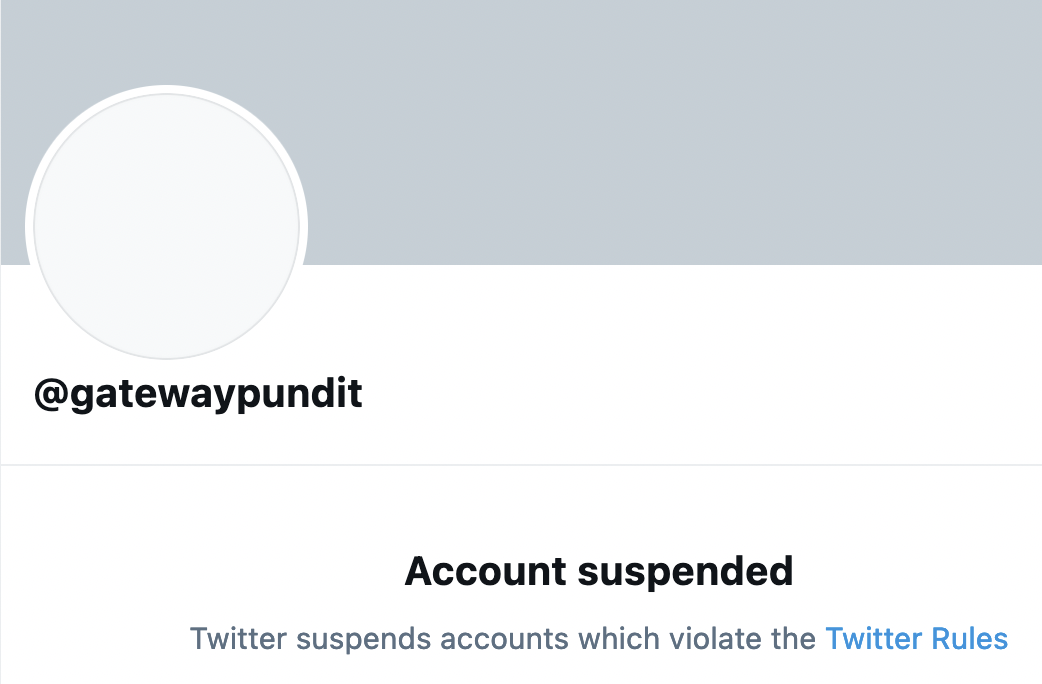
\includegraphics[scale=0.2]{./img/fig1.png}  \hfill 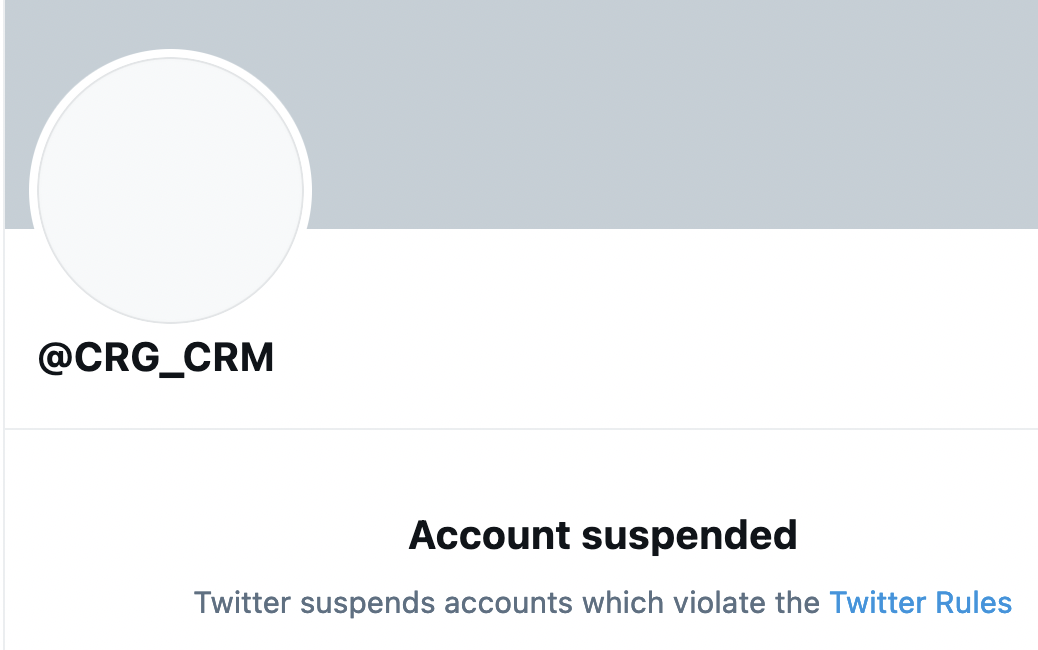
\includegraphics[scale=0.2]{./img/crg.png} \hfill 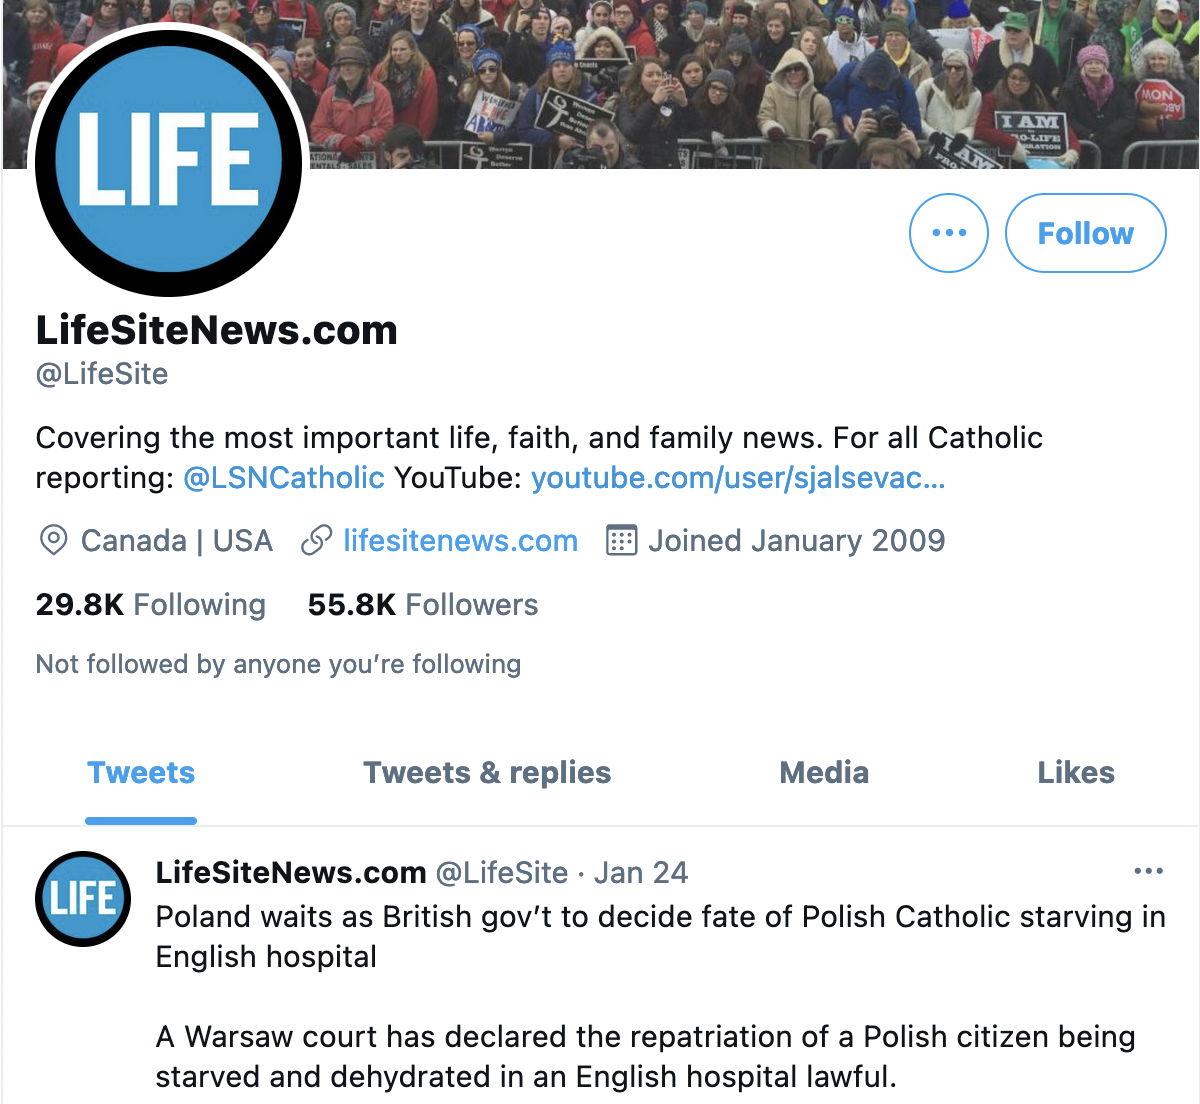
\includegraphics[scale=0.2]{./img/life.png} 
%\caption{Screenshots taken on June 14, 2021 at 4pm UTC. }
%\label{fig1}
%\end{figure}

\smallskip

\subsubsection{Twitter}

%\begin{figure}
%\centering
%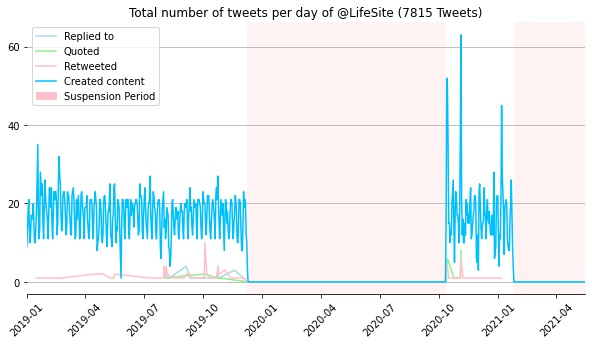
\includegraphics[scale=0.35]{./img/lifesite.jpg} 
%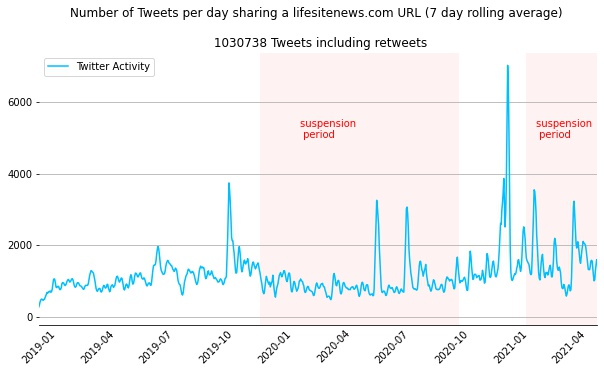
\includegraphics[scale=0.35]{./img/lifesite_rolling_7_lifesite.jpg}
%\caption{Panel (a): number of Tweets per day of the Twitter account $@Lifesite$ linked to the website lifesitenews.com from January, 2019 until April 2021. Panel (b): number of Tweets per day that have shared a lifesitenews.com URL link from January, 2019 until April 2021. }
%\label{fig2}
%\end{figure}

\begin{figure}
\centering
\begin{multicols}{1}
    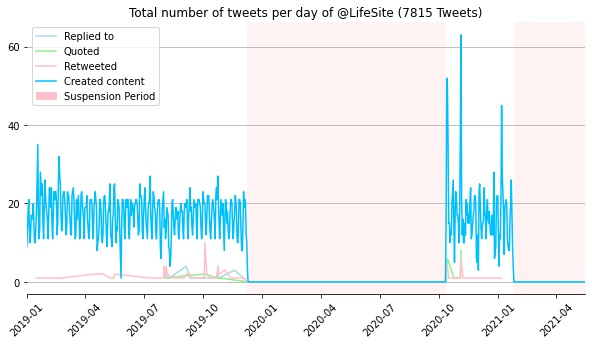
\includegraphics[scale=0.32]{./img/lifesite.jpg}\par 
    %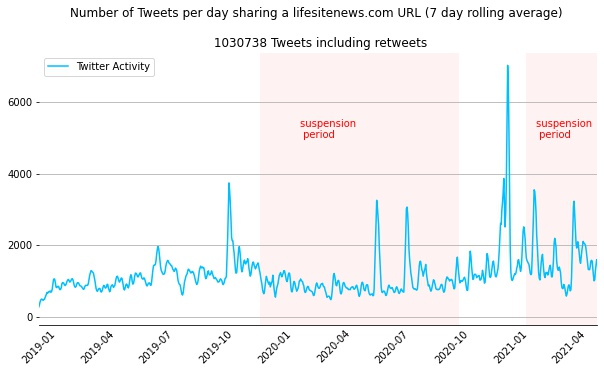
\includegraphics[width=\linewidth]{./img/lifesite_rolling_7_lifesite.jpg}\par 
    \end{multicols}
\begin{multicols}{1}
   % 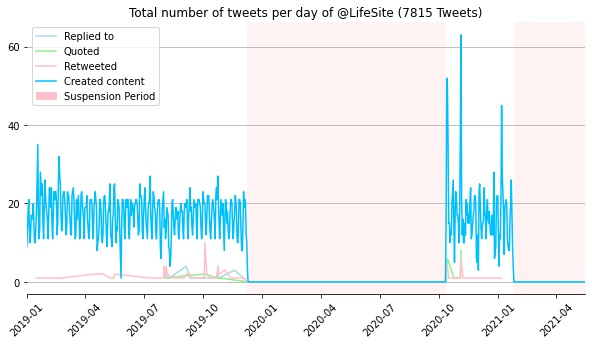
\includegraphics[width=\linewidth]{./img/lifesite.jpg}\par
    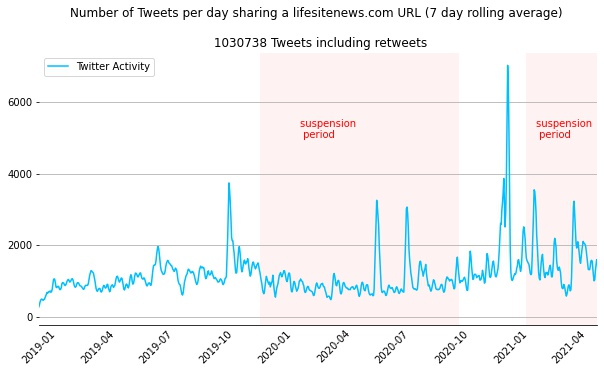
\includegraphics[scale=0.32]{./img/lifesite_rolling_7_lifesite.jpg}\par
\end{multicols}
\caption{Panel (a): number of Tweets per day of the Twitter account $@Lifesite$ linked to the website lifesitenews.com from January, 2019 until April 2021. Panel (b): number of Tweets per day that have shared a lifesitenews.com URL link from January, 2019 until April 2021.}
\label{fig2}
\end{figure}


In this section, we discuss one case of temporary suspension on Twitter.\footnote{See the official documentation on the Twitter's Help Center regarding account suspension: \href{https://help.twitter.com/en/managing-your-account/suspended-twitter-accounts}{https://help.twitter.com/en/managing-your-account/suspended-twitter-accounts }.} The Twitter account of the website lifesitenews.com has been suspended for at least two periods of time: from end of 2019 until fall 2020 for 308 days, then again since January 2021 for having violated Twitter Rules\footnote{See Lifesitenews's article discussing the reason of the suspension: \href{https://www.lifesitenews.com/news/lifesite-is-dumping-twitter-and-so-should-you}{https://www.lifesitenews.com/news/lifesite-is-dumping-twitter-and-so-should-you}. Twitter rules can be found at: \href{https://help.twitter.com/en/rules-and-policies/twitter-rules}{https://help.twitter.com/en/rules-and-policies/twitter-rules}. }. In particular, this website has several failed fact-checks concerning the published articles, according to Iffy.news.\footnote{See \href{https://mediabiasfactcheck.com/life-site-news/}{https://mediabiasfactcheck.com/life-site-news/}}. We collected the activity (tweets, replies, quotes, retweets) on their Twitter account $@LifeSite$ via the Twitter API, using the historical search endpoint.\footnote{See the documentation: \href{https://developer.twitter.com/en/docs/twitter-api/tweets/search/api-reference/get-tweets-search-all}{https://developer.twitter.com/en/docs/twitter-api/tweets/search/api-reference/get-tweets-search-all}.} We then plotted the number of Tweets, Retweets, Quotes and Replies per day, as shown in panel $a$ of figure \ref{fig2}). The two periods of temporary suspension are clearly observed in the data as the user(s) of the account were not allowed to use the functionalities of the Twitter Platform. 

\smallskip

To further assess the impact of this double temporary suspension, we collect via Minet Command Line Tool\cite{minet}, all the tweets that have shared during the same period a url link containing lifesitenews.com. Panel $(b)$ of figure \ref{fig2}, shows that during both periods of temporary suspension, other users still shared lifesitenews.com links and that the level was only slightly below the tweeting and retweeting levels prior to the first temporary suspension. More specifically, there was an average of 960 tweets (including retweets) per day over the first temporary suspension period of 308 days from December 9, 2019 until October 12, 2020, against an average of 977 tweets (including retweets) per day during the exact same period one year earlier. Finally, panel $(b)$ points towards the limitations of suspending an account to limit the spread of its content. 

\subsubsection{Facebook}

Unfortunately when an account is permanently suspended by Facebook, it disappears from the platform (so its data cannot be scrapped anymore), and its data also disappears from the CrowdTangle API.\footnote{CrowdTangle is a public insights tool owned and operated by Facebook, that exclusively tracks public content from Facebook public groups and pages.} For a previous research project\footnote{reference?}, we searched on CrowdTangle for public accounts sharing specific content associated with misinformation in November $2020$, and selected $94$ Facebook pages corresponding to our criteria. We then tried to collect these pages' posts in January $2021$, and discovered that $11$ pages could not be found anymore. This highlights an important issue when studying misinformation trends on Facebook: some data disappears from the CrowdTangle API as accounts are deleted or changed to {\it private}.

Interestingly, Facebook is regularly publishing a monthly {\it coordinated inauthentic behavior} report where it informs how many personal accounts, pages or groups were deleted and to which {\it deceptive network} they may have belonged.\footnote{See the April 2021 report for an example: \href{https://about.fb.com/news/2021/05/april-2021-coordinated-inauthentic-behavior-report/}{https://about.fb.com/news/2021/05/april-2021-coordinated-inauthentic-behavior-report/}} But as long as external persons do not have access to deleted accounts data, these reports cannot be verified by independent researchers or journalists.

Facebook can also apply a temporary suspension, and in this case the data can often be collected and analyzed. For example, \href{https://www.facebook.com/DonaldTrump/}{Donald Trump’s official Facebook page}  has been suspended following the Capitol attack on January 6, 2021.\footnote{See \href{https://www.facebook.com/zuck/posts/10112681480907401}{https://www.facebook.com/zuck/posts/10112681480907401}} Nevertheless the page’s data is still present in the CrowdTangle API. Thus, after manually adding this page to the CrowdTangle dashboard, we collected the $6$ $083$ posts it published between January $1$, $2020$ and June $15$, $2021$ using the {\it posts} endpoint.\footnote{ (see the endpoint documentation for more details: \href{https://github.com/CrowdTangle/API/wiki/Posts}{https://github.com/CrowdTangle/API/wiki/Posts}.} We used the minet command line tool \cite{minet} to collect data. We can verify on figure \ref{fig1_fb} that the {\it Donald J. Trump} page has not published any content since January $6$, 2021, and that this behavior is not consistent with the page’s previous activity: an average of $16$ posts were published each day on Facebook before the suspension. 


%\begin{figure}
%	\centering
%	%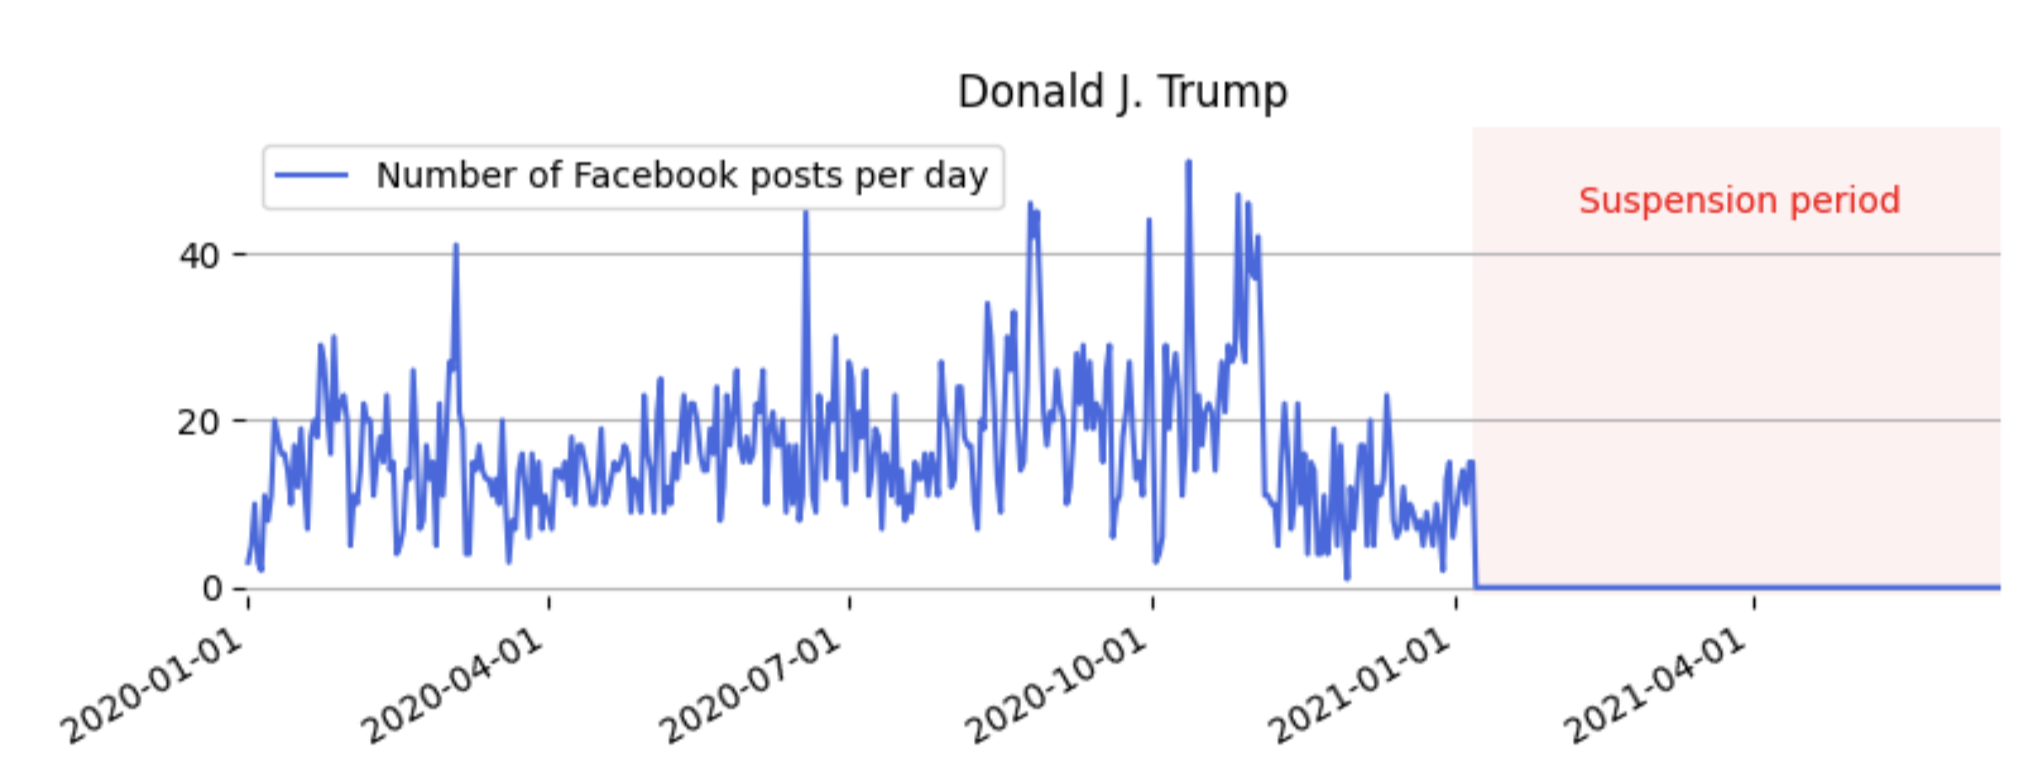
\includegraphics[scale=0.35]{./img/fb/fig1_fb.png}
%	\caption{Number of Facebook posts published each day by the Facebook page {\it Donald J. Trump} between January $1$, $2020$ and June $15$, $2021$. The data corresponds to $6$ $083$ posts retrieved from the CrowdTangle API using the {\it posts} endpoint.}
%	\label{fig1_fb}
%\end{figure}

\begin{figure}
\begin{multicols}{1}
    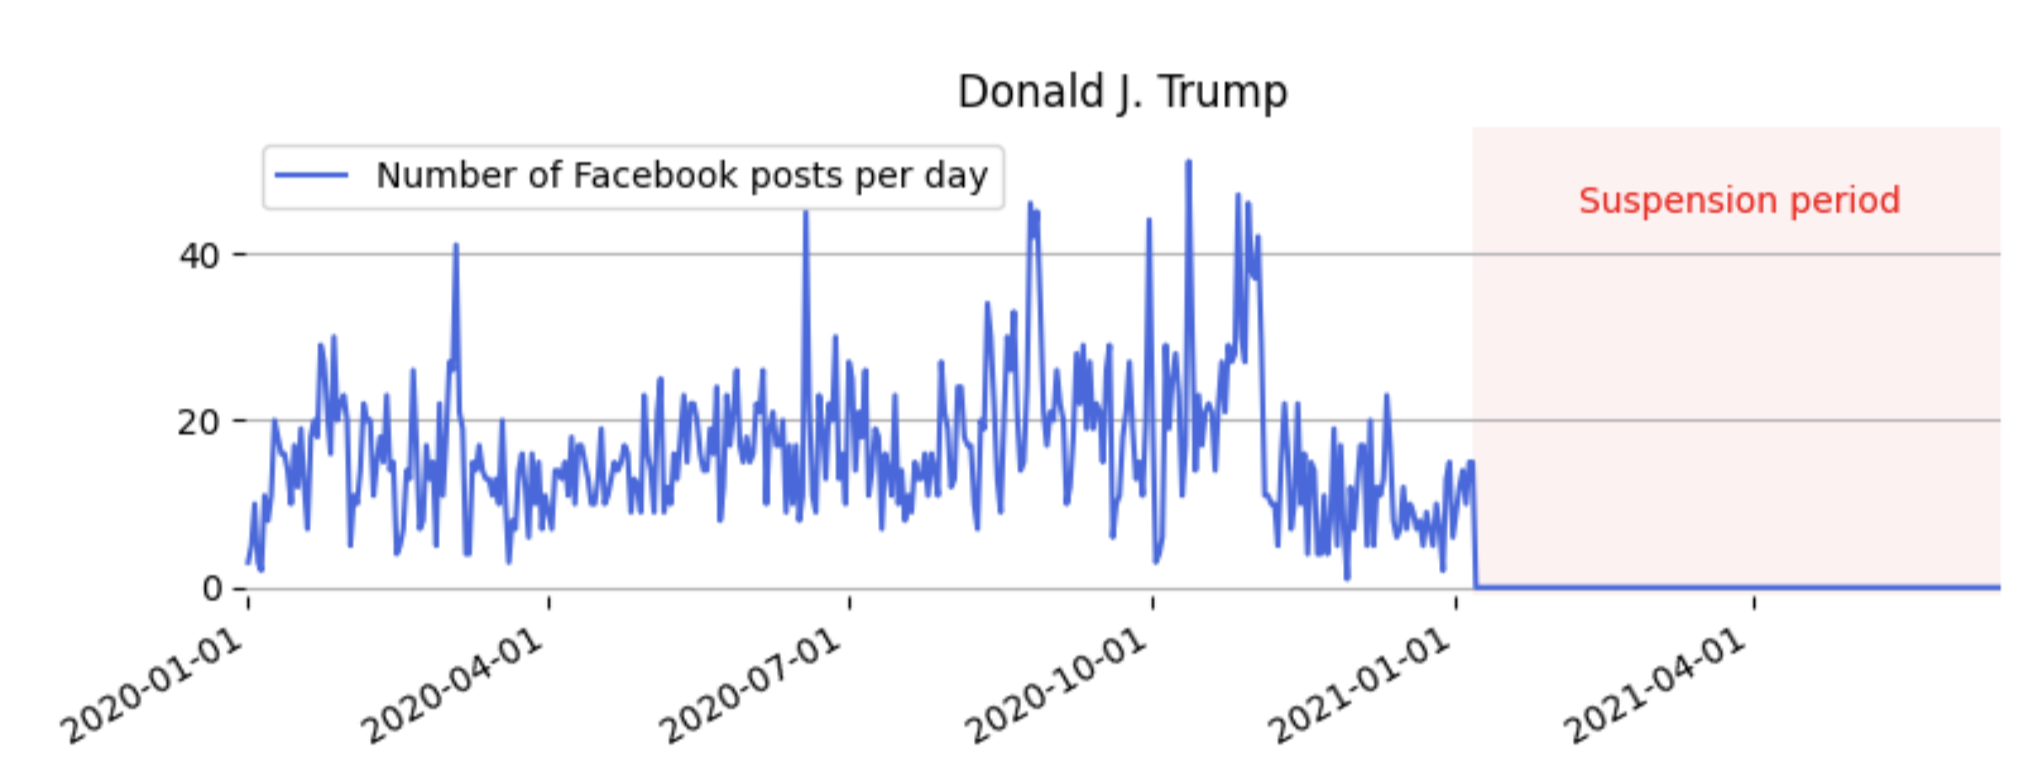
\includegraphics[scale=0.22]{./img/fb/fig1_fb.png}\par 
   % 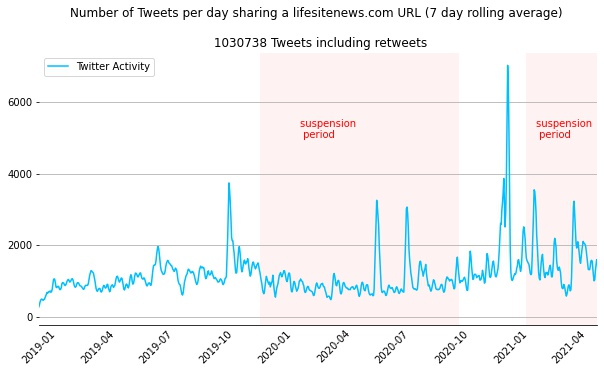
\includegraphics[width=\linewidth]{./img/lifesite_rolling_7_lifesite.jpg}\par 
    \end{multicols}
%\begin{multicols}{2}
   % 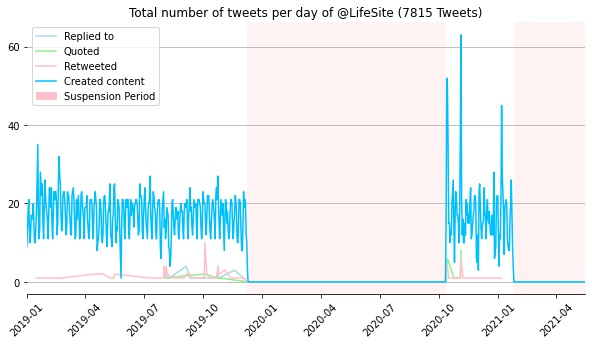
\includegraphics[width=\linewidth]{./img/lifesite.jpg}\par
 %   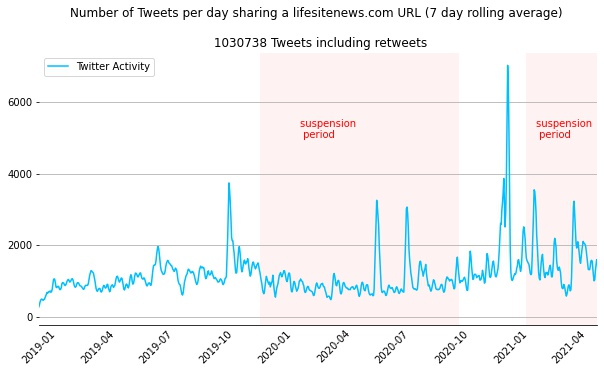
\includegraphics[width=\linewidth]{./img/lifesite_rolling_7_lifesite.jpg}\par
%\end{multicols}
\caption{Number of Facebook posts published each day by the Facebook page {\it Donald J. Trump} between January $1$, $2020$ and June $15$, $2021$. The data corresponds to $6$ $083$ posts retrieved from the CrowdTangle API using the {\it posts} endpoint.}
\label{fig1_fb}
\end{figure}



\subsubsection{Youtube}

In this section, we turn to the channel temporary or permanent suspension policy of Youtube. Whenever a channel publishes a video that violates the community guidelines for the first time they will  usually receive a warning and the content will be removed. For the second time the channel will start receiving strikes. A first strike results in limiting the access of the Youtube channel  for one week, like uploading videos, streaming and other activities. Then a second strike is similar but the suspension will be for two weeks. A third strike results in the termination of the channel. The strike count of a channel lasts 90 days.  In the special case, where a video is in extreme violation of the guidelines, the publishing channel may get terminated without a warning.\footnote{See the ``Community Guidelines strike basics''. Youtube help, Google Developers,  \href{https://support.google.com/youtube/answer/2802032?hl=en. Accessed 21 6 2021}{https://support.google.com/youtube/answer/2802032?hl=en. Accessed 21 6 2021}.} To illustrate the implementation of this policy we provide two examples for the temporary suspension of the following two Youtube channels: \href{https://www.youtube.com/channel/UCNbIDJNNgaRrXOD7VllIMRQ}{One America news Network} and \href{https://www.youtube.com/user/TonyHeller1}{Tony Heller}.

\smallskip

%\begin{figure}
%	\centering
%	%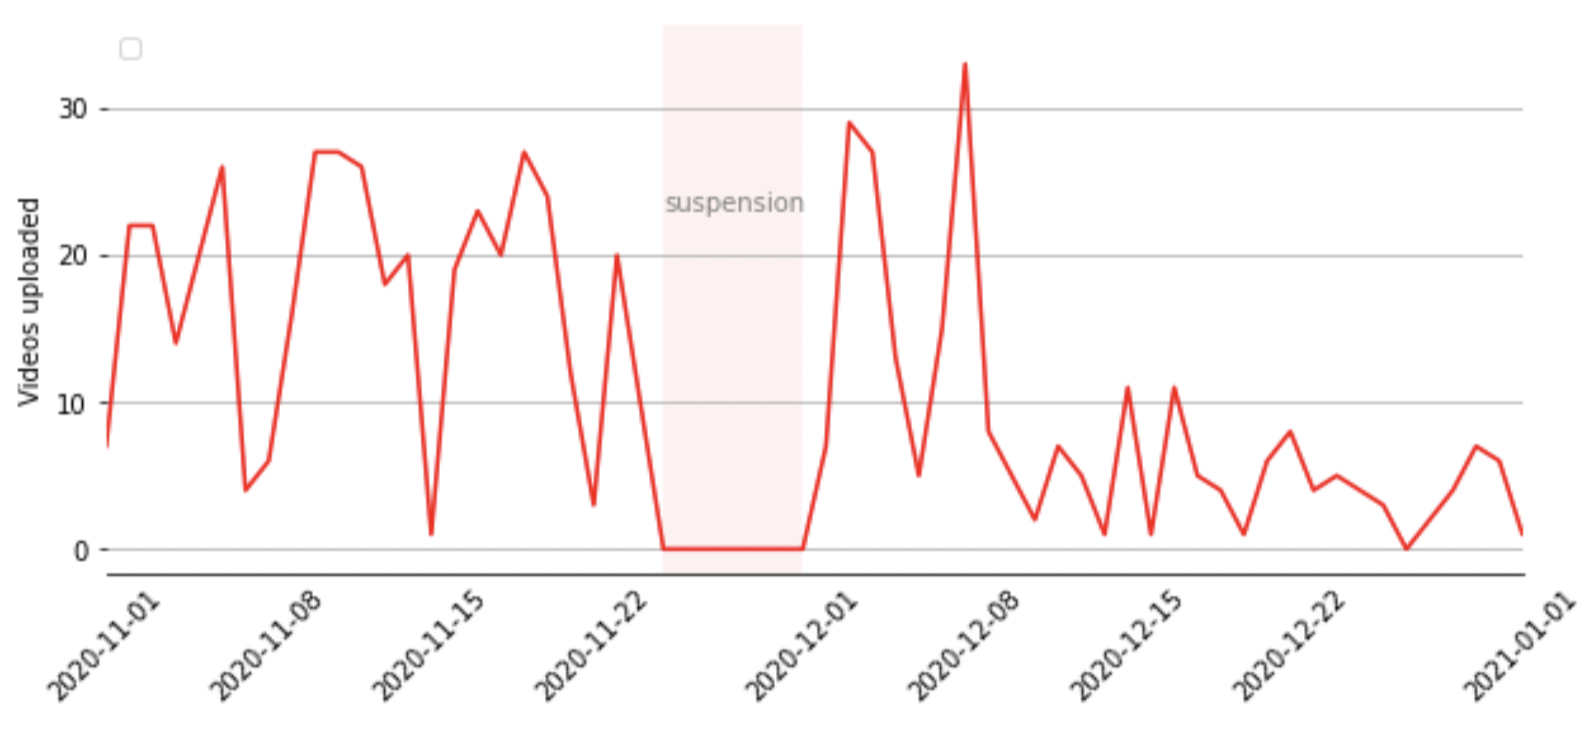
\includegraphics[scale=0.25]{./img/oann/fig1_oann.png}
%	%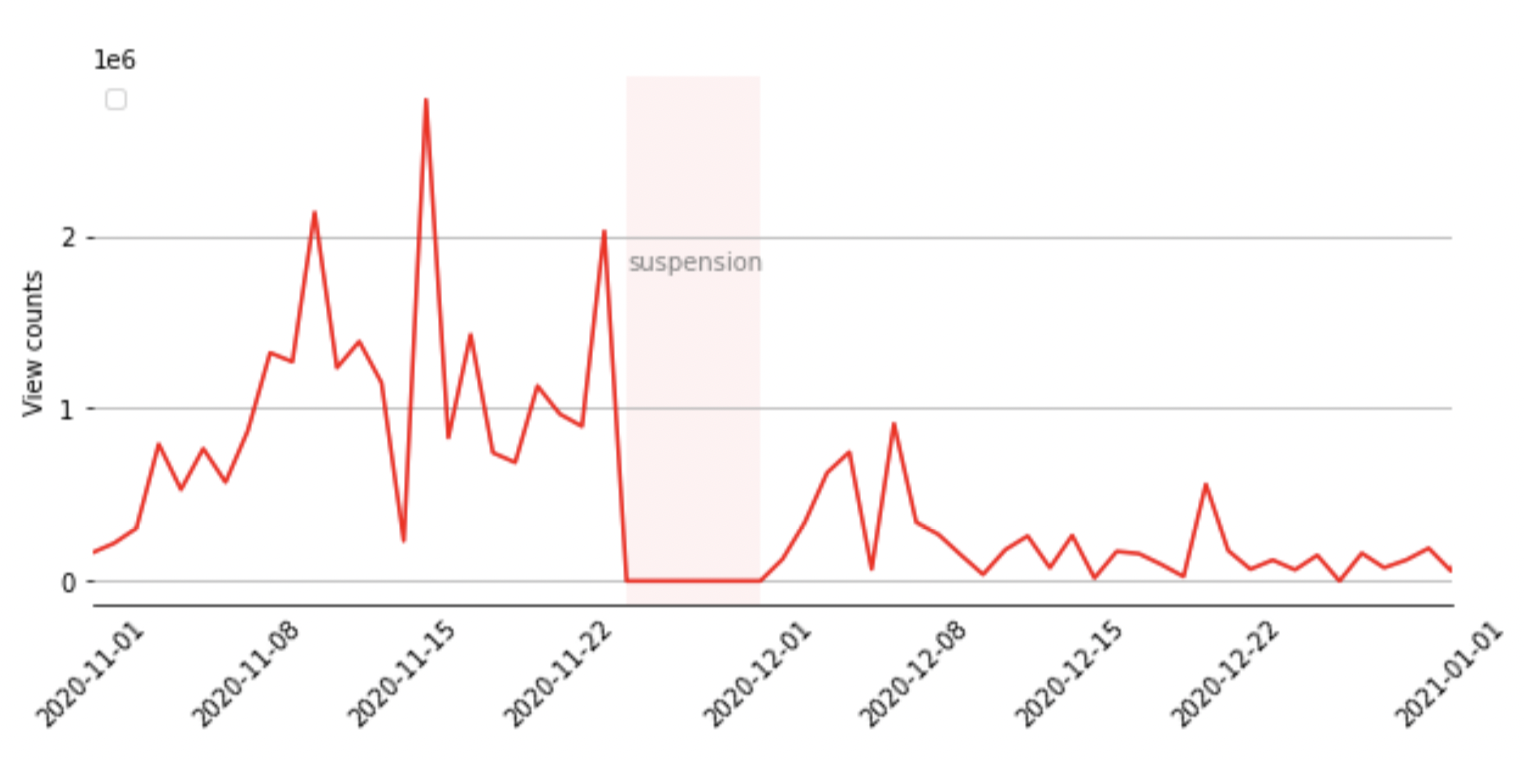
\includegraphics[scale=0.25]{./img/oann/fig2_oann.png} 
%	\caption{panel (a): Number of Youtube videos uploaded each day by the youtube channel {\it One America news Network} November 1, 2020 and January 1, 2021. Panel (b): accumulated view counts for videos. The metrics correspond to the videos’  publishing date and the data is retrieved from the youtube API with the {\it playlists} and  {\it videos} endpoints. }
%	\label{fig1_oann}
%\end{figure}


\begin{figure}
\centering
\begin{multicols}{1}
    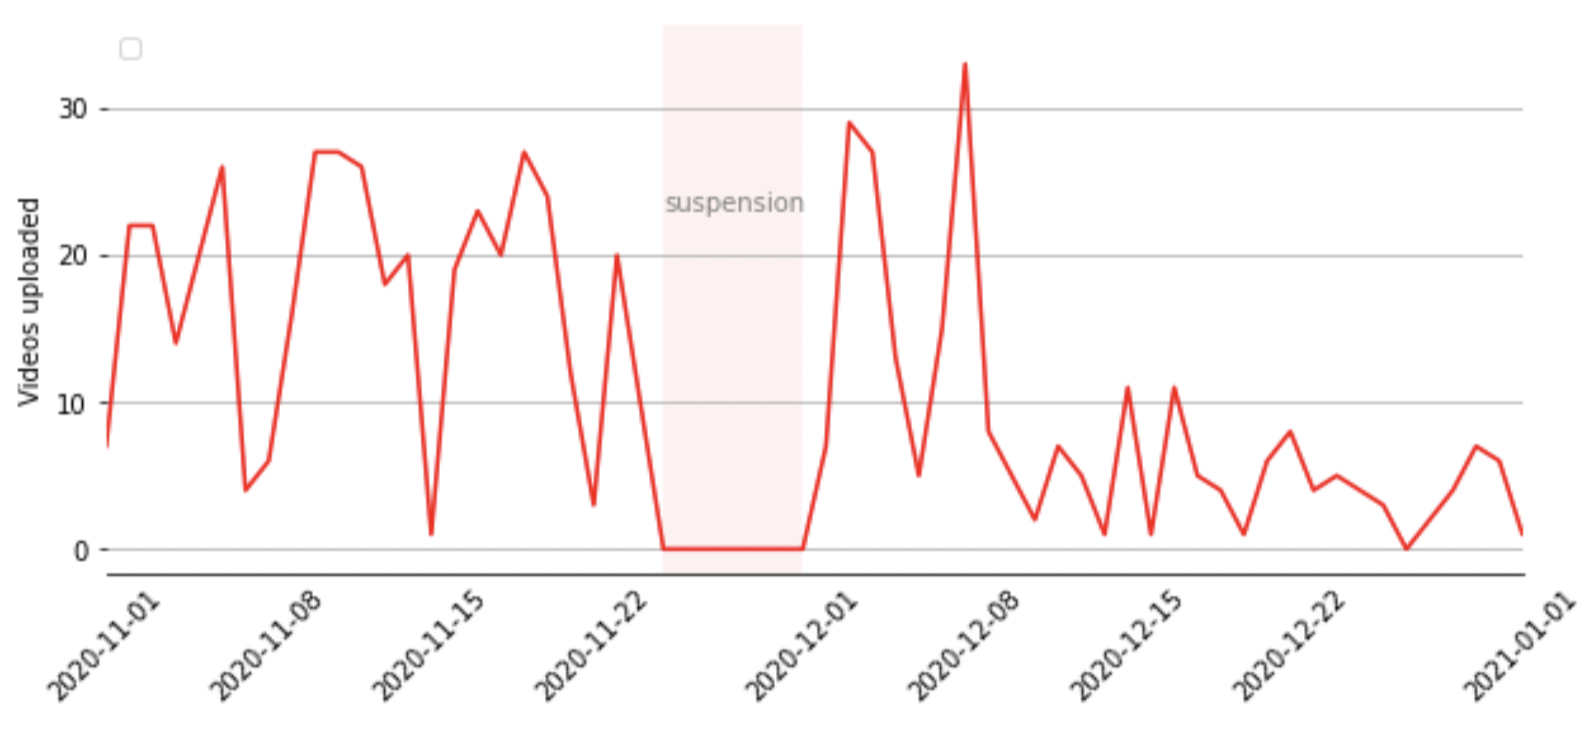
\includegraphics[scale=0.3]{./img/oann/fig1_oann.png}\par 
    %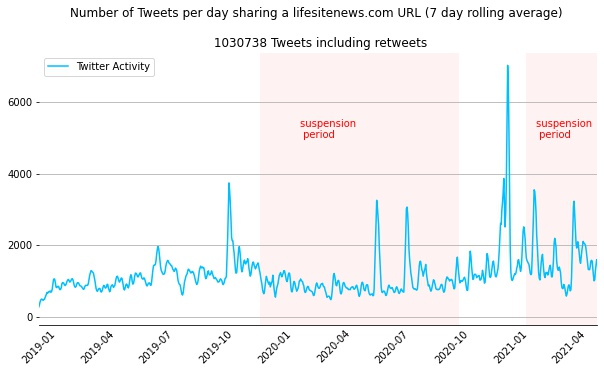
\includegraphics[width=\linewidth]{./img/lifesite_rolling_7_lifesite.jpg}\par 
    \end{multicols}
\begin{multicols}{1}
   % 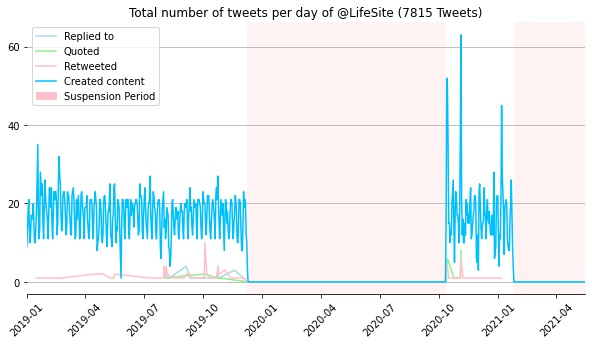
\includegraphics[width=\linewidth]{./img/lifesite.jpg}\par
    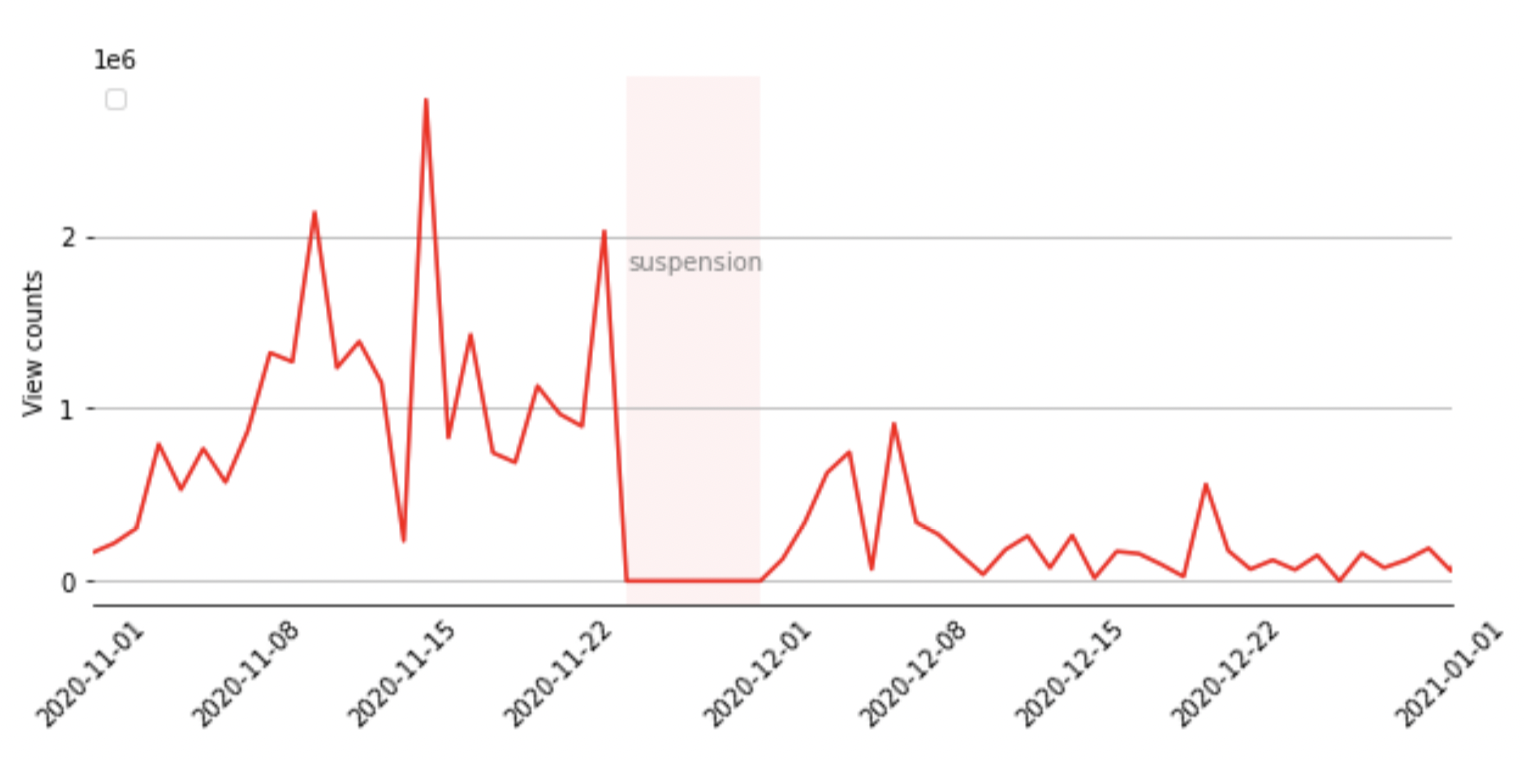
\includegraphics[scale=0.3]{./img/oann/fig2_oann.png}\par
\end{multicols}
\caption{panel (a): Number of Youtube videos uploaded each day by the youtube channel {\it One America news Network} November 1, 2020 and January 1, 2021. Panel (b): accumulated view counts for videos. The metrics correspond to the videos’  publishing date and the data is retrieved from the youtube API with the {\it playlists} and  {\it videos} endpoints. }
\label{fig1_oann}
\end{figure}

First, we investigate the temporary suspension case of the Youtube Channel of {\it One America News channel}. This channel received a first strike on November 24, 2020 for the promotion of  a false cure for COVID19.\footnote{Reference?} We collected the activity of the channel OANN (video counts, view counts) using  the Youtube API v3, between November 2020 and January 2021. For the video counts, we used the playlist endpoint to retrieve the videos uploaded with their publishing date and for the view count we used the IDs of the videos we had from the playlists and via the videos endpoint we retrieved the view counts on June 2021.\footnote{See the Google documentation  \href{https://developers.google.com/youtube/v3/docs/videos/list}{https://developers.google.com/youtube/v3/docs/videos/list} and \href{https://developers.google.com/youtube/v3/docs/playlists/list}{https://developers.google.com/youtube/v3/docs/playlists/list}} 

\smallskip



In addition, as shown in figure \ref{fig1_oann} when comparing the week before the suspension from 2020/11/17 to 2020/11/23 and one week after from 2020/12/01 to 2020/12/07 it was found that the view count had decreased by ($-45\%$ or $-60\%$), even though the posted number of videos was similar (before $81$ videos; after 93 videos or 86 videos). In other words, the suspension period may have a good impact on reducing the audience interest or reach to the channel. Besides that, OANN decided to move officially to Rumble on March 17, 2021 as announced on their Twitter account (see figure \ref{fig2_oann}) and their upload activity on their Youtube channel is close to zero since that announcement. 

%\begin{figure}
%	\centering
%	%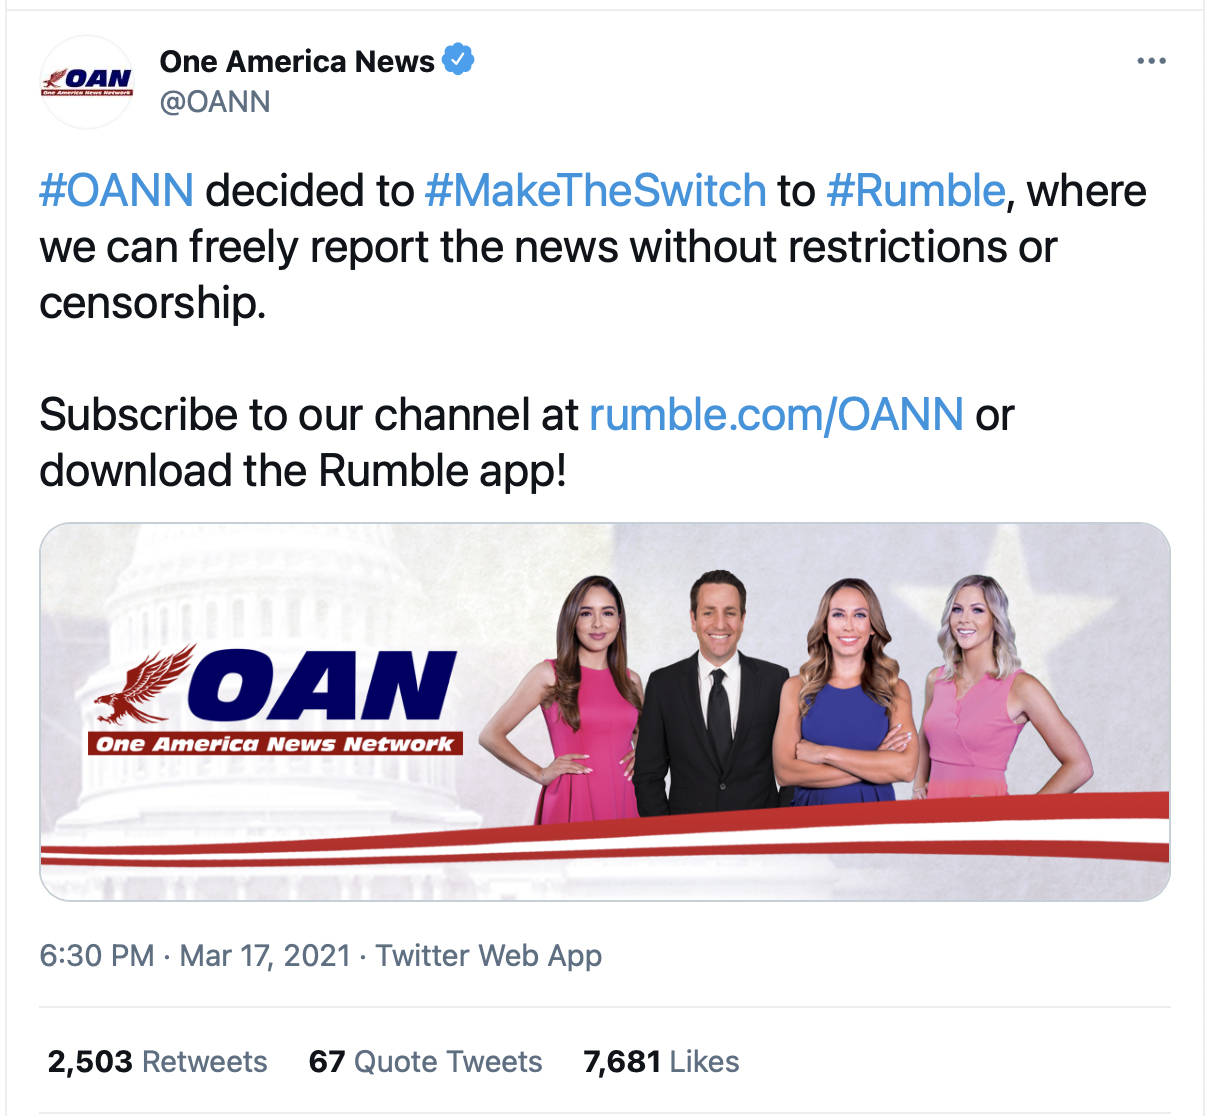
\includegraphics[scale=0.2]{./img/oann/fig3_oann.png}
%	%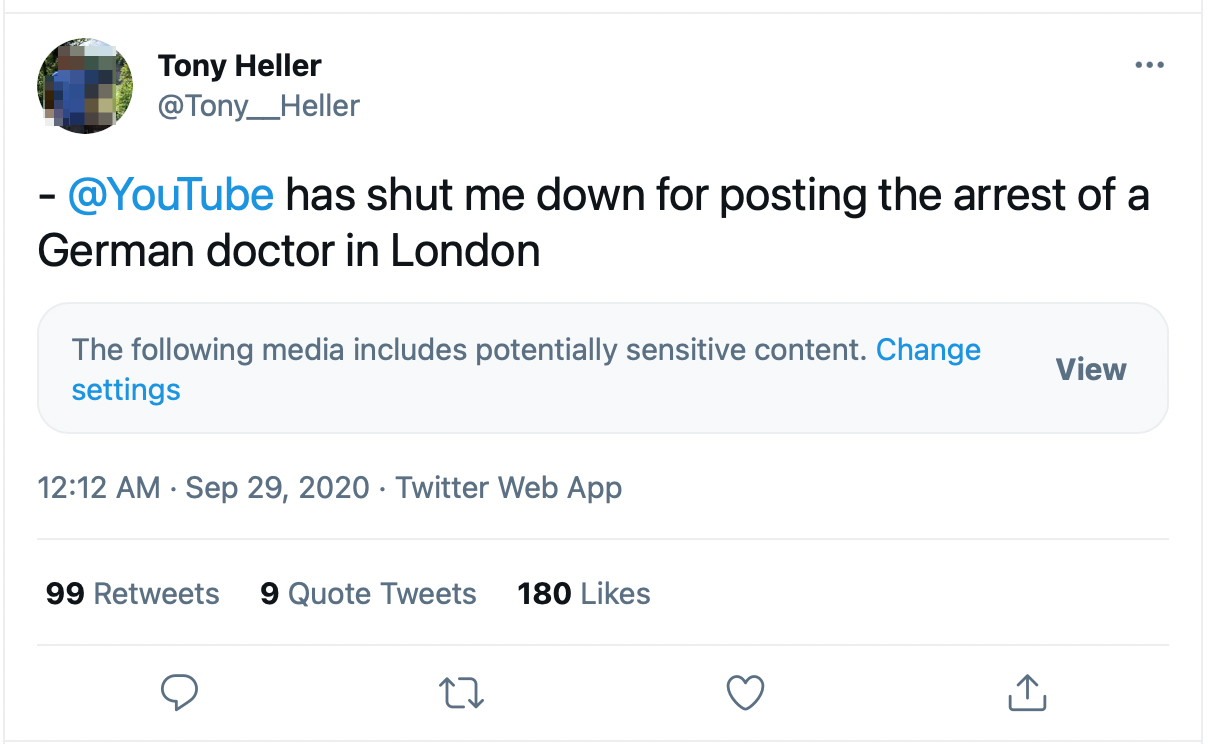
\includegraphics[scale=0.3]{./img/tony/fig3_tony.png}
%	\caption{Panel (a): Tweet announcing moving to rumble by OANN (Twitter), see: \href{https://twitter.com/OANN/status/1372238828425998336}{https://twitter.com/OANN/status/1372238828425998336}. Panel (b): Tony Heller's tweet after getting suspended from Youtube, see \href{https://twitter.com/Tony\_Heller/status/1310703852769796097}{https://twitter.com/Tony\_Heller/status/1310703852769796097}.}
%	\label{fig2_oann}
%\end{figure}



\begin{figure}
\centering
\begin{multicols}{1}

    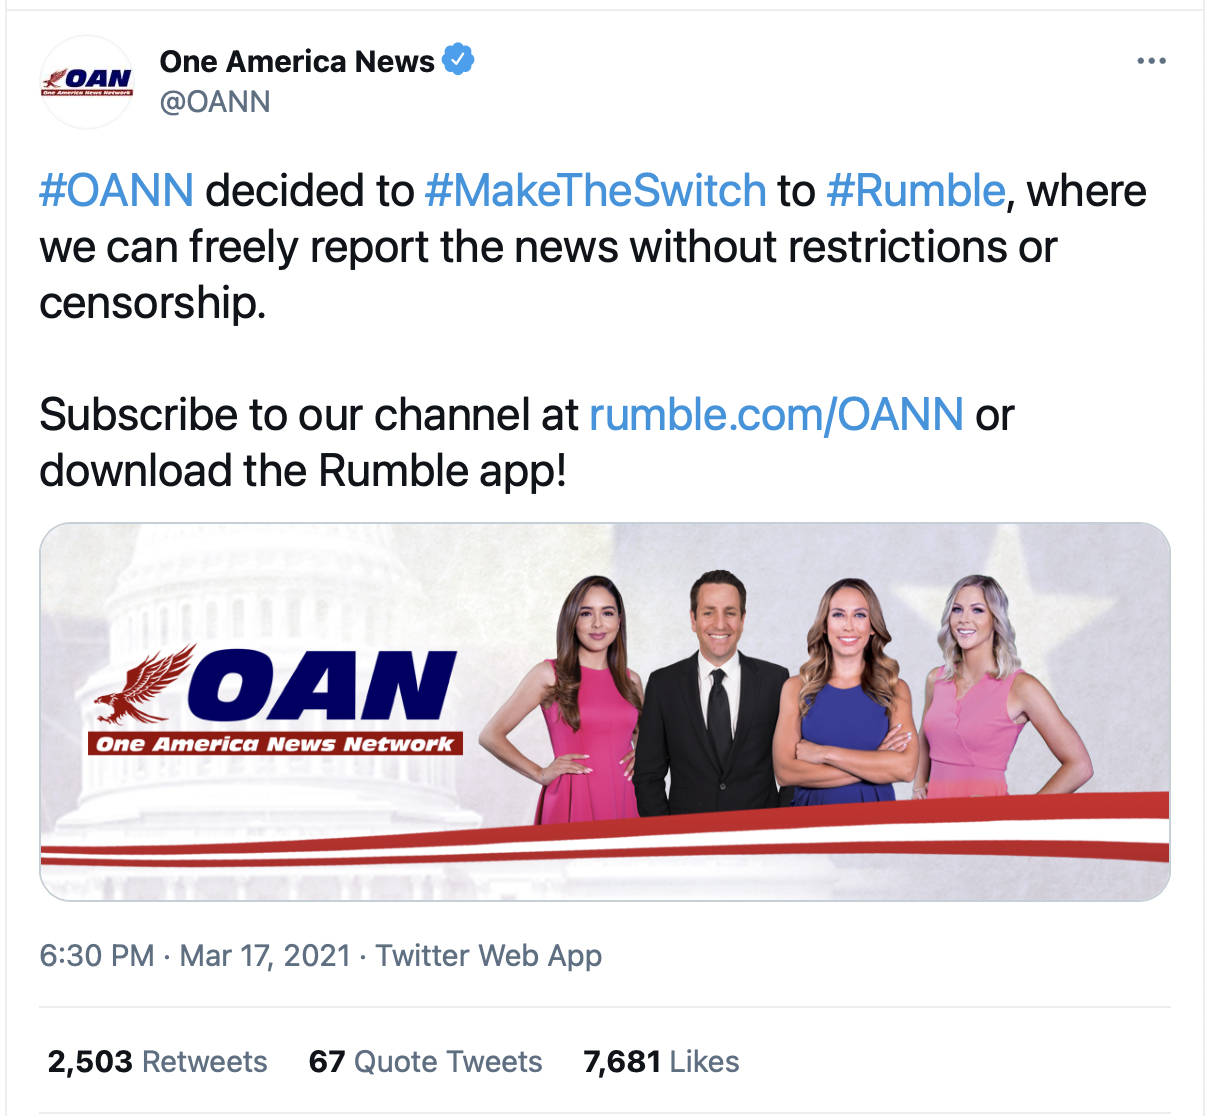
\includegraphics[scale=0.25]{./img/oann/fig3_oann.png}\par 
    %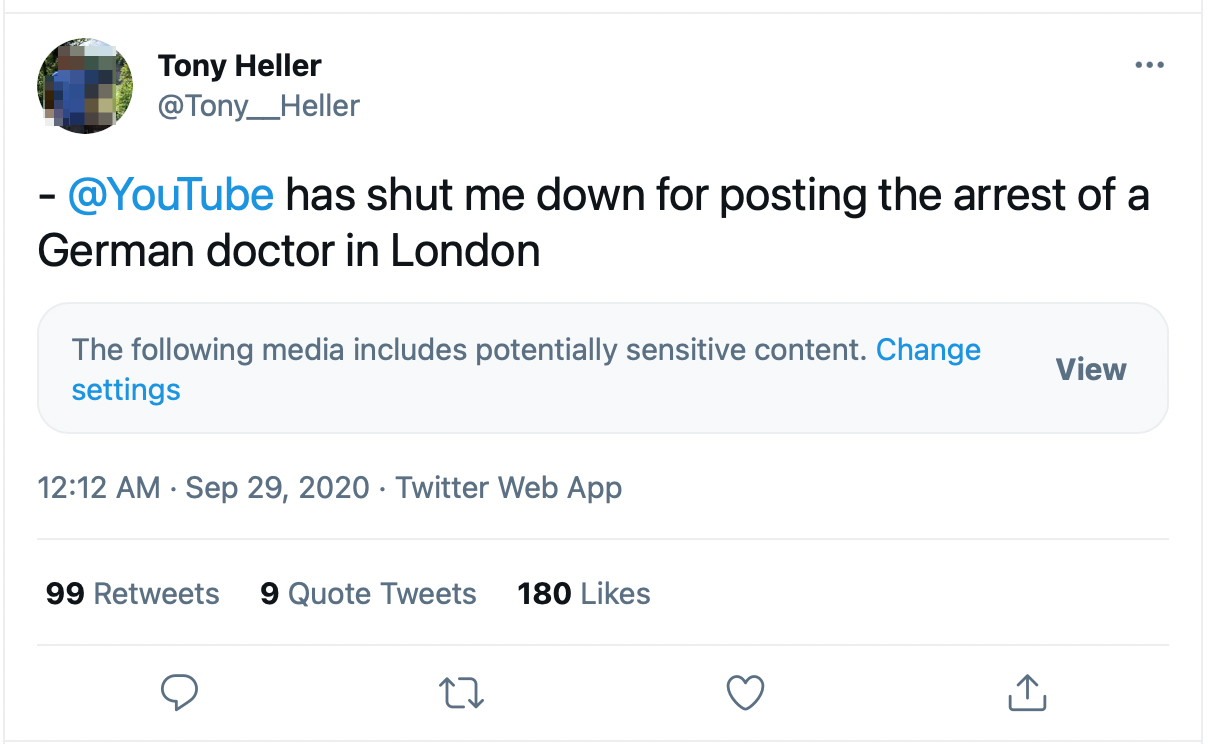
\includegraphics[scale=0.2]{./img/tony/fig3_tony.png}\par 
    \end{multicols}
\begin{multicols}{1}

   % 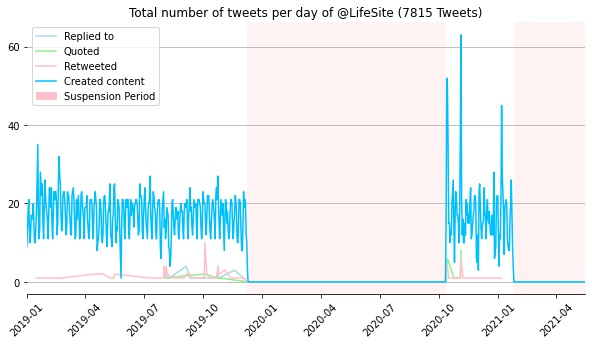
\includegraphics[width=\linewidth]{./img/lifesite.jpg}\par
    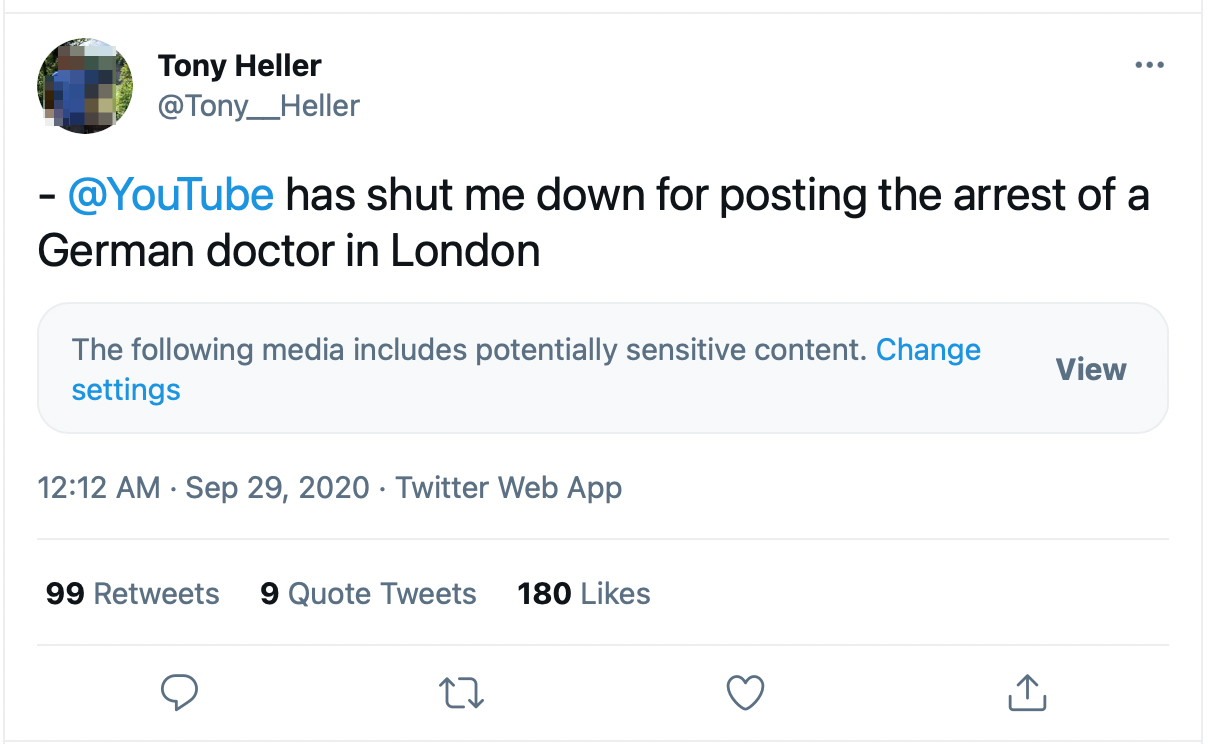
\includegraphics[scale=0.25]{./img/tony/fig3_tony.png}\par
\end{multicols}
\caption{Panel (a): Tweet announcing moving to rumble by OANN (Twitter), tweet ID \href{https://twitter.com/OANN/status/1372238828425998336}{1372238828425998336}. Panel (b): Tony Heller's tweet after getting suspended from Youtube, tweet ID \href{https://twitter.com/Tony\_Heller/status/1310703852769796097}{1310703852769796097}. }
\label{fig2_oann}
\end{figure}


\smallskip


We now turn to our second example, the temporary suspension of the Youtube channel Tony Heller. This channel got its first strike after posting a video about an anti-covid-lockdown doctor getting arrested (see screenshot in figure \ref{fig2_oann}). The suspension period was for one week from September 29 until October 5. We applied the same methods as in the previous example for the data collection. Figure \ref{fig2_oann} shows the daily number of videos uploaded by the channel. The suspension period can be observed clearly in the historical data of the channel. Moreover, observing the reach of the audience using view counts one week before the suspension starting from 2020/09/22 to 2020/09/28 and one week after the suspension from 2020/10/06 to 2020/10/12 the channel witnessed a drop of $-65\%$ and the videos published in the channel were less by $-16\%$.

%\begin{figure}
%	\centering
%	%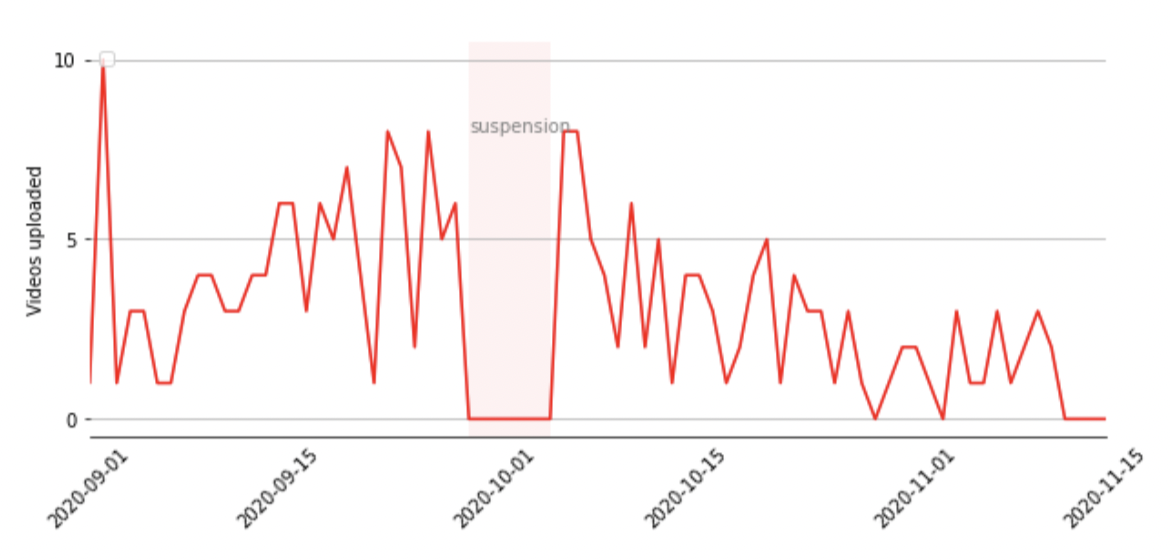
\includegraphics[scale=0.3]{./img/tony/fig1_tony.png}
%	%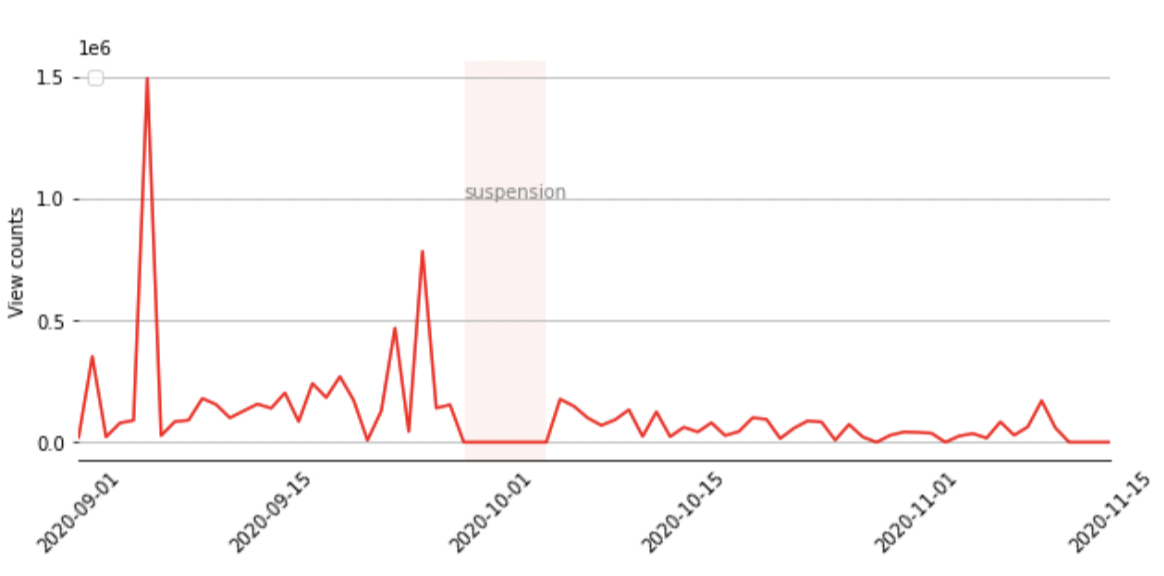
\includegraphics[scale=0.3]{./img/tony/fig2_tony.png}
%	\caption{Panel (a): Number of Youtube videos uploaded each day by the Youtube channel {\it Tony Heller} between September 1, 2020 and November 15, 2020. Panel (b): accumulated view counts for videos uploaded by the same Youtube channel. The date corresponds to the videos’  publishing date. 
%}
%	\label{fig1_tony}
%\end{figure}


\begin{figure}
\centering
\begin{multicols}{1}

    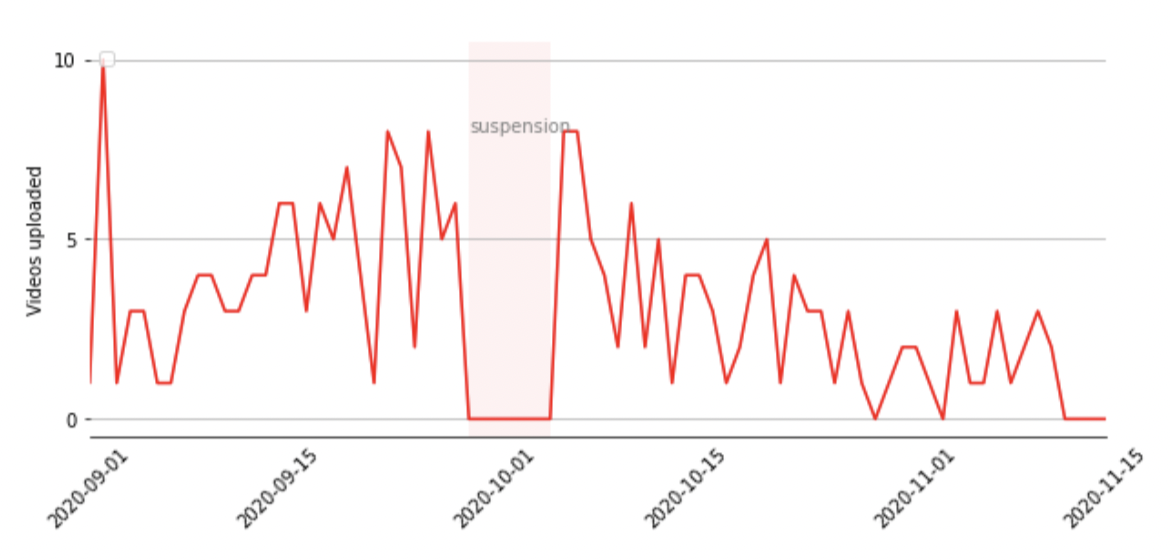
\includegraphics[scale=0.33]{./img/tony/fig1_tony.png}\par 
    %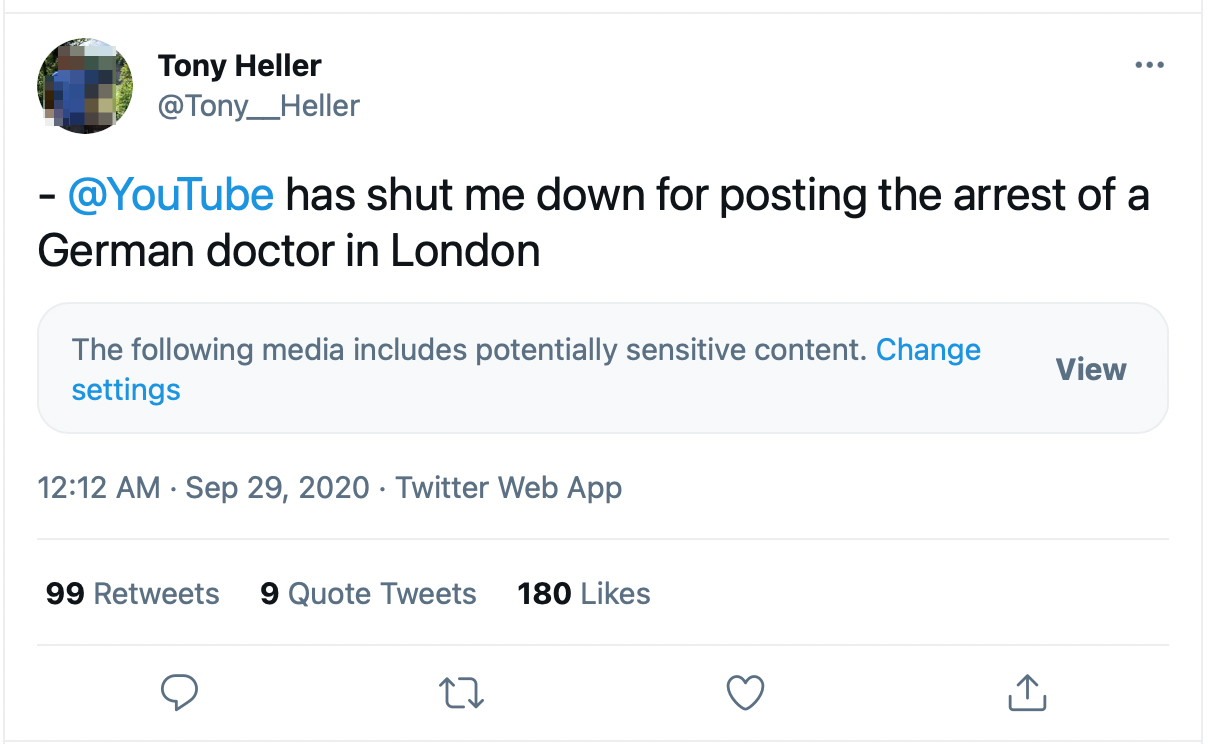
\includegraphics[scale=0.2]{./img/tony/fig3_tony.png}\par 
    \end{multicols}
\begin{multicols}{1}

   % 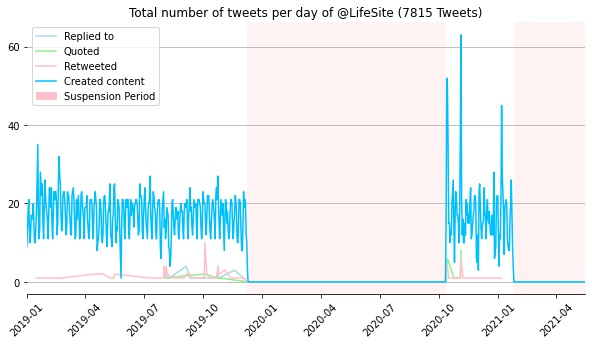
\includegraphics[width=\linewidth]{./img/lifesite.jpg}\par
    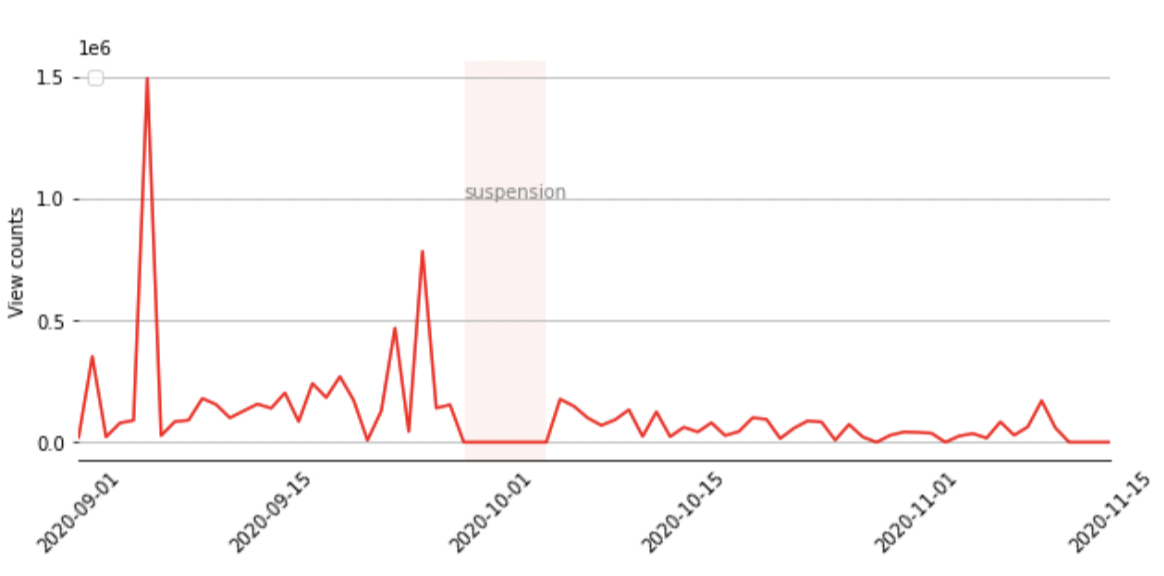
\includegraphics[scale=0.33]{./img/tony/fig2_tony.png}\par
\end{multicols}
\caption{Panel (a): Number of Youtube videos uploaded each day by the Youtube channel {\it Tony Heller} between September 1, 2020 and November 15, 2020. Panel (b): accumulated view counts for videos uploaded by the same Youtube channel. The date corresponds to the videos’  publishing date. 
 }
\label{fig2_oann}
\end{figure}


\subsection{Blocking links}

A third measure that main stream social media platforms can apply is to prevent users from sharing specific types of content, instead of deleting the content after posting, or users accounts. We will study here how the platforms prevent users from sharing urls coming from specific domain names.

\subsubsection{Facebook}

The Beauty of life

\subsection{Reducing the visibility}

Mainstream Social Media platforms can reduce the visibility of the content created or shared by specific users, whenever they violate the platforms' rules. The implementation of this policy varies accros platforms and is not easy to verify ex-post. In what follows we provide means to verify this policy on Twitter and Facebook.  

\subsubsection{Facebook}

Infowars 

\subsubsection{Twitter} 

%\begin{figure}
%	\centering
%	%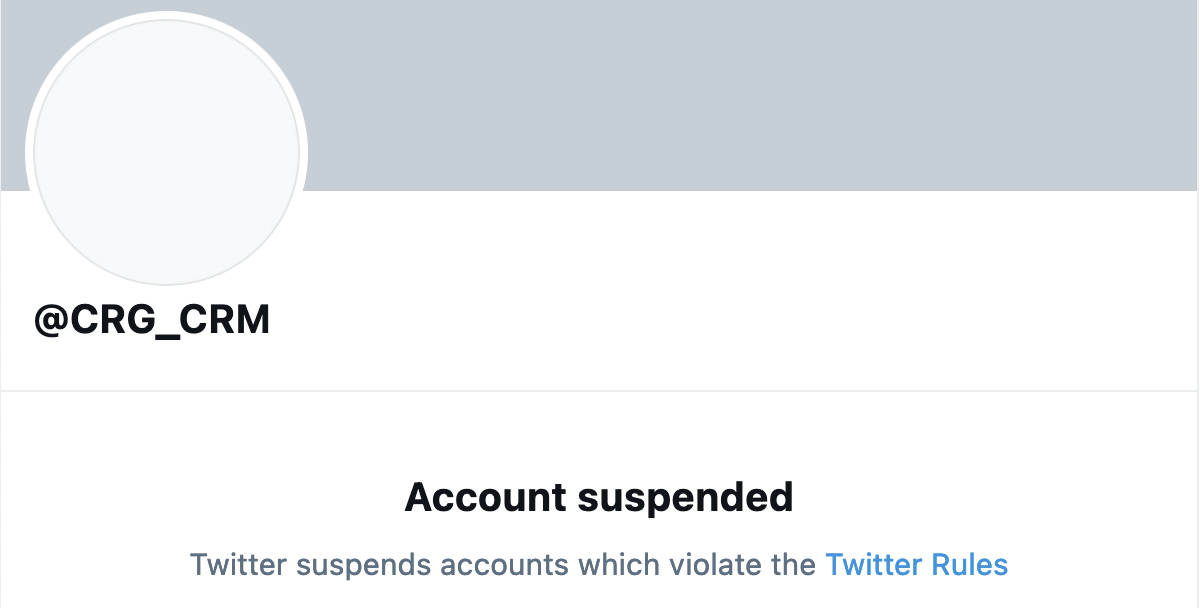
\includegraphics[scale=0.3]{./img/globalresearch_2021-06-14.png}
%	%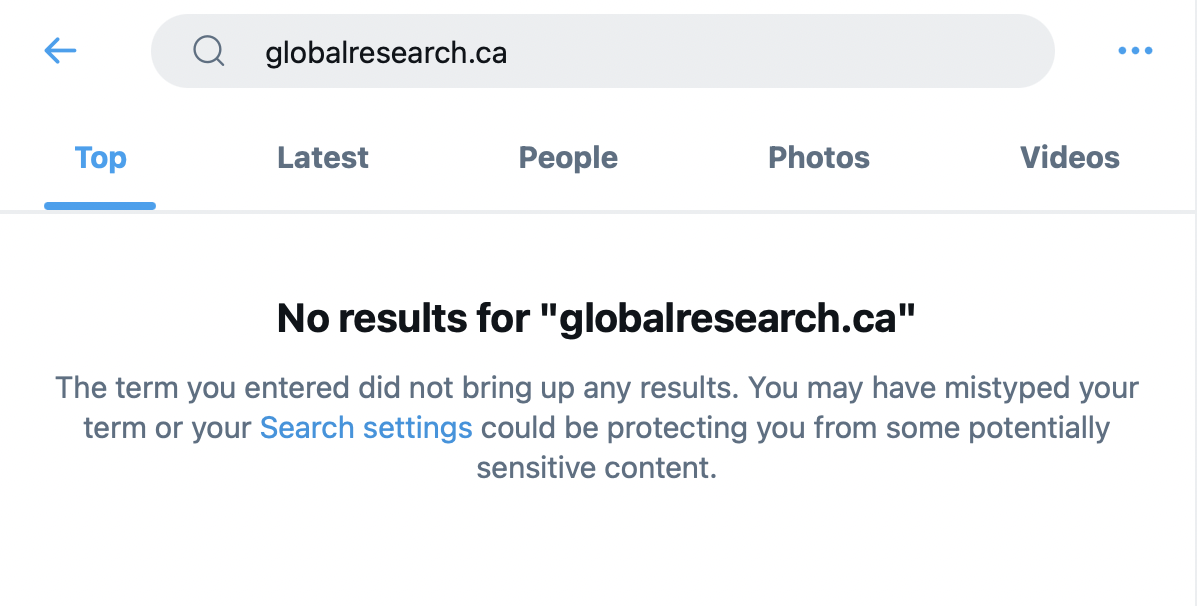
\includegraphics[scale=0.3]{./img/globalresearch_14_06_2021_16pm_UTC.png} 
%	\caption{Screenshots taken on June 14, 2021. }
%	\label{fig3}
%\end{figure}


%\begin{figure}
%\centering
%\begin{multicols}{1}
%
%    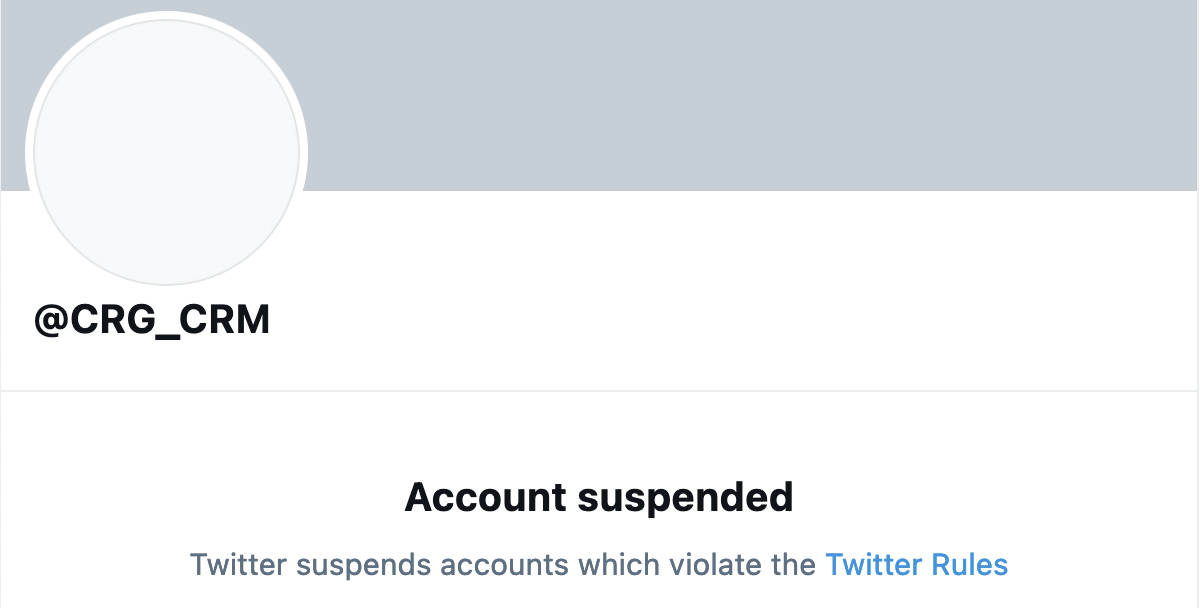
\includegraphics[scale=0.33]{./img/globalresearch_2021-06-14.png}\par 
%    %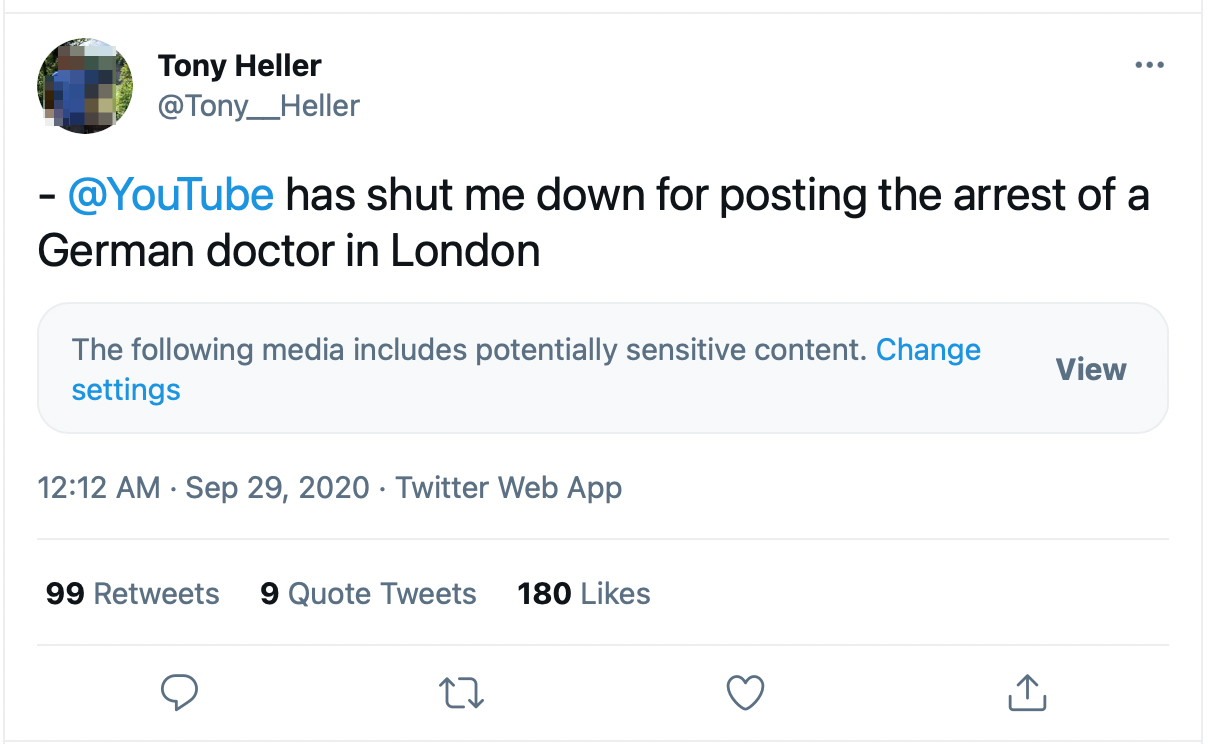
\includegraphics[scale=0.2]{./img/tony/fig3_tony.png}\par 
%    \end{multicols}
%\begin{multicols}{1}
%
%   % 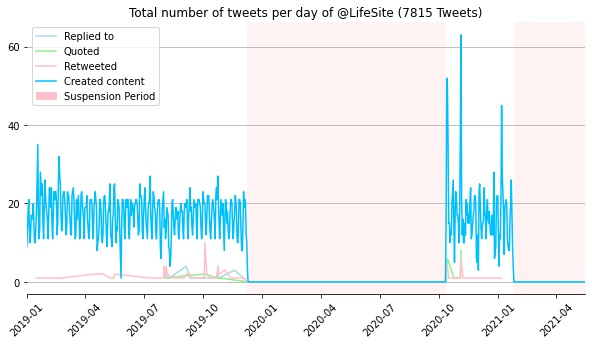
\includegraphics[width=\linewidth]{./img/lifesite.jpg}\par
%    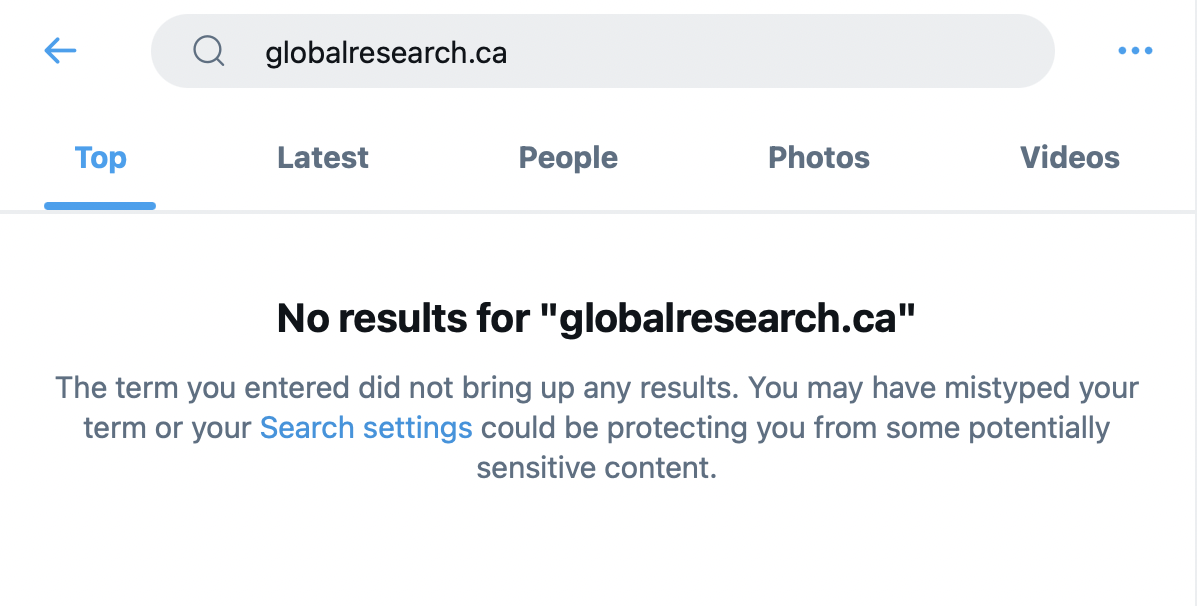
\includegraphics[scale=0.33]{./img/globalresearch_14_06_2021_16pm_UTC.png}\par
%\end{multicols}
%\caption{Screenshots taken on June 14, 2021. 
% }
%\label{fig3}
%\end{figure}



Twitter can take action against a tweet which violates the Twitter rules\footnote{See the paragraph {\it Limiting Tweet visibility}: \href{https://help.twitter.com/en/rules-and-policies/enforcement-options}{https://help.twitter.com/en/rules-and-policies/enforcement-options}.}, by limiting its visibility on users' timelines and in search results. To illustrate we provide an example for the website $globalresearch.ca$, which has several failed fact-checks according to \href{https://iffy.news}{iffy.news} - a website which provides a database of websites with low factual reporting levels.\footnote{For $globalresearch.ca$ see \href{https://mediabiasfactcheck.com/global-research/}{https://mediabiasfactcheck.com/global-research/} .  }

\smallskip

%To illustrate we provide two examples linked to the Twitter accounts of the websites $globalresearch.ca$ and $off$-$guardian.org$. Both websites have several failed fact-checks according to \href{https://iffy.news}{iffy.news} - a website which provides a database of websites with low factual reporting levels.\footnote{For $globalresearch.ca$ see \href{https://mediabiasfactcheck.com/global-research/}{https://mediabiasfactcheck.com/global-research/} and for $off-guardian.org$ see \href{https://mediabiasfactcheck.com/offguardian/}{https://mediabiasfactcheck.com/offguardian/}.  }

The website $globalresearch.ca$ is linked to the Twitter account {$@CRG\_CRM$}; that was recently suspended.\footnote{We noticed the message about the account suspension on May 25, 2021. But to the best of our knowledge, no official communication by Twitter has announced the suspension nor the exact date at which it was implemented. Hence the account may have gotten suspended anytime between April 15, 2021 and May 25, 2021 (see the suspension screenshot in panel $(a)$ of figure \ref{fig3}). Furthermore, $globalresearch.ca$ has multiple failed fact-checks, see \href{https://mediabiasfactcheck.com/global-research/}{https://mediabiasfactcheck.com/global-research/}} When a user searches via the twitter search-box a url link of this website, no results appear as shown in the screenshot in panel $(b)$ of figure \ref{fig3}, taken on June 14, 2021. To further investigate the possible implementation of a reduced visibility measure, we search via the Twitter API for tweets, excluding retweets, containing the query {\it globalresearch.ca} from January 1, 2021 until June 10, 2021.  As shown in panel (a) in figure \ref{fig4}, we find a strictly positive number of tweets containing the URL link {\it globalresearch.ca} throughout May 2021 and the first week of June 2021. Hence, the visibility of tweets containing this URL link has been reduced because users can no longer access tweets containing the URL link {\it globalresearch.ca} via the search box. Nevertheless users are not restrained from posting tweets containing this URL, as shown in the screenshot in panel $(c)$
 of figure \ref{fig4}, found by taking the tweet ID of one of the collected tweets via the Twitter API. Furthermore, those collected Tweets have strictly positive engagement metrics as shown in panel $(b)$ of figure \ref{fig4}. Hence, the users who tweet articles from the {\it globalresearch.ca} website receive positive engagement from their own followers. Finally, when a user attempts to click on the URL link {\it globalresearch.ca} contained in the Tweet, a warning message appears and indicates that the link may be unsafe (see screenshot in panel (d) in figure \ref{fig4}). 


%\begin{figure}
%\centering
%%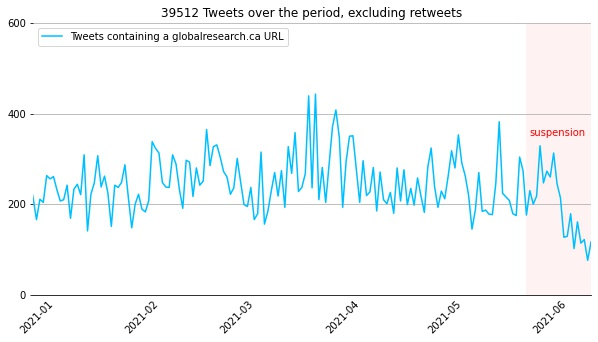
\includegraphics[scale=0.3]{./img/globalresearch/sum_globalresearch.ca_6_months.jpg} 
%%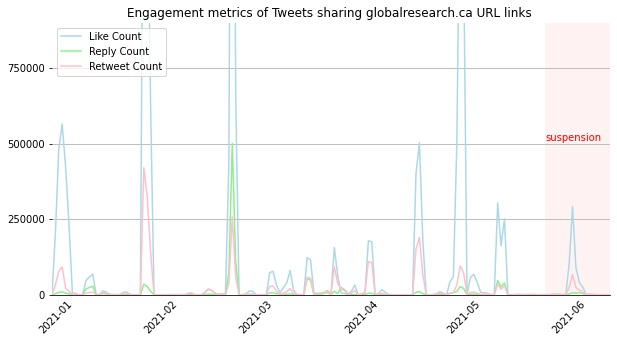
\includegraphics[scale=0.3]{./img/globalresearch/engagement_sum_rolling_1_globalresearch.ca.jpg}
%%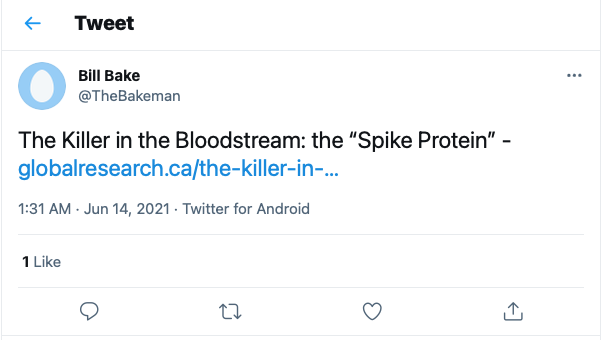
\includegraphics[scale=0.3]{./img/globalresearch/tweet.png} 
%%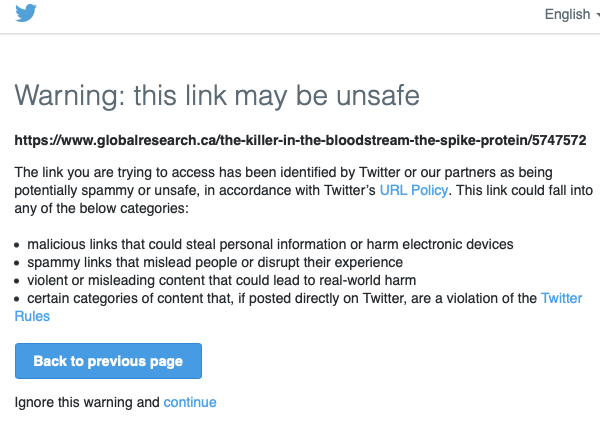
\includegraphics[scale=0.3]{./img/globalresearch/warning.png}
%\caption{Panel (a):}
%\label{fig4}
%\end{figure}

%\begin{figure}
%\centering
%\begin{multicols}{1}
%
%    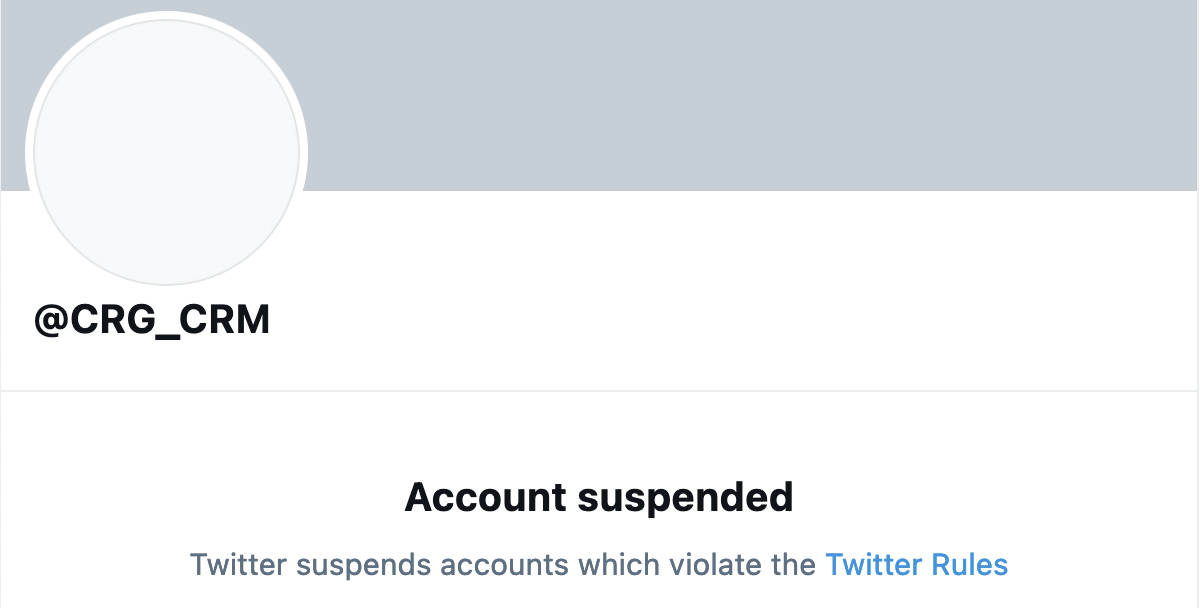
\includegraphics[scale=0.33]{./img/globalresearch_2021-06-14.png}\par 
%    %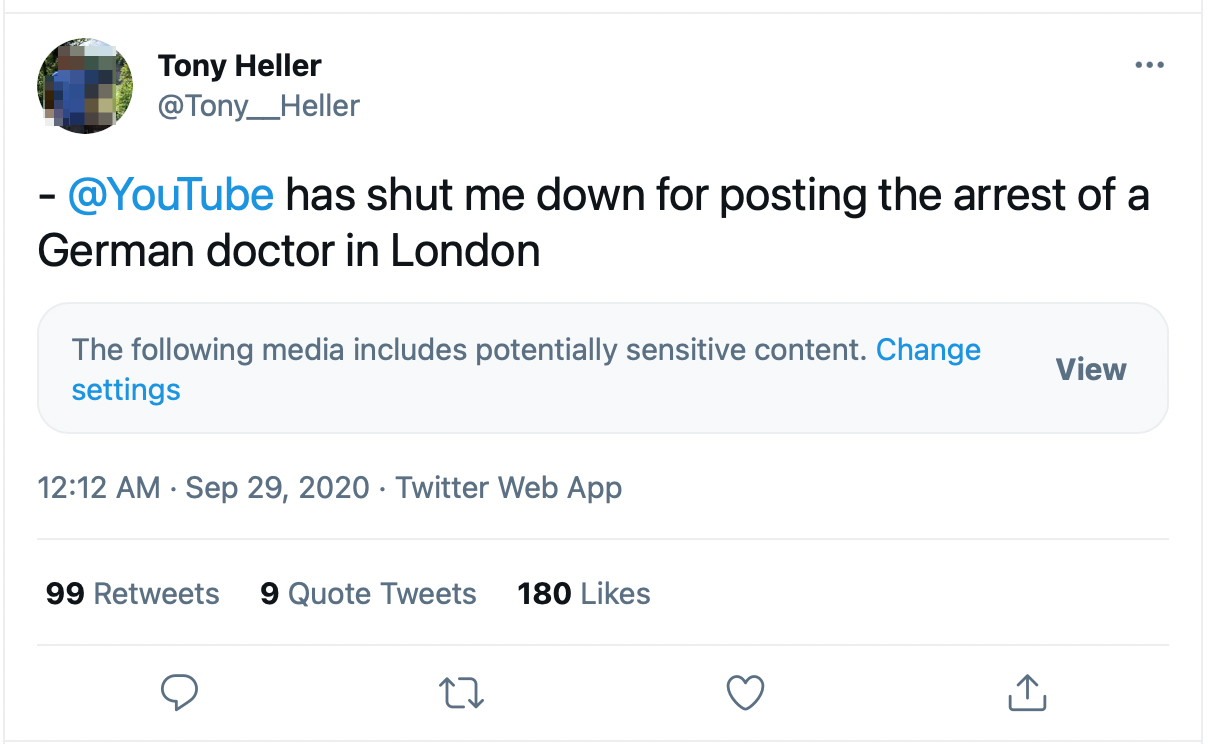
\includegraphics[scale=0.2]{./img/tony/fig3_tony.png}\par 
%    \end{multicols}
%\begin{multicols}{1}
%
%   % 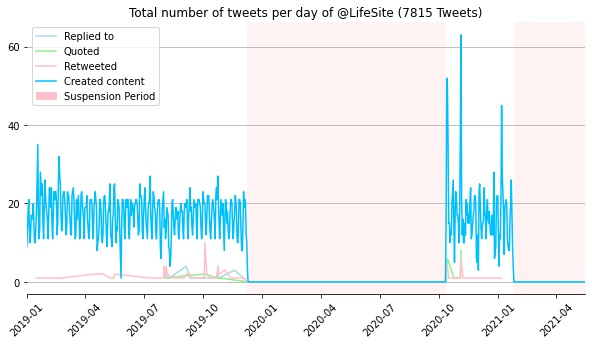
\includegraphics[width=\linewidth]{./img/lifesite.jpg}\par
%    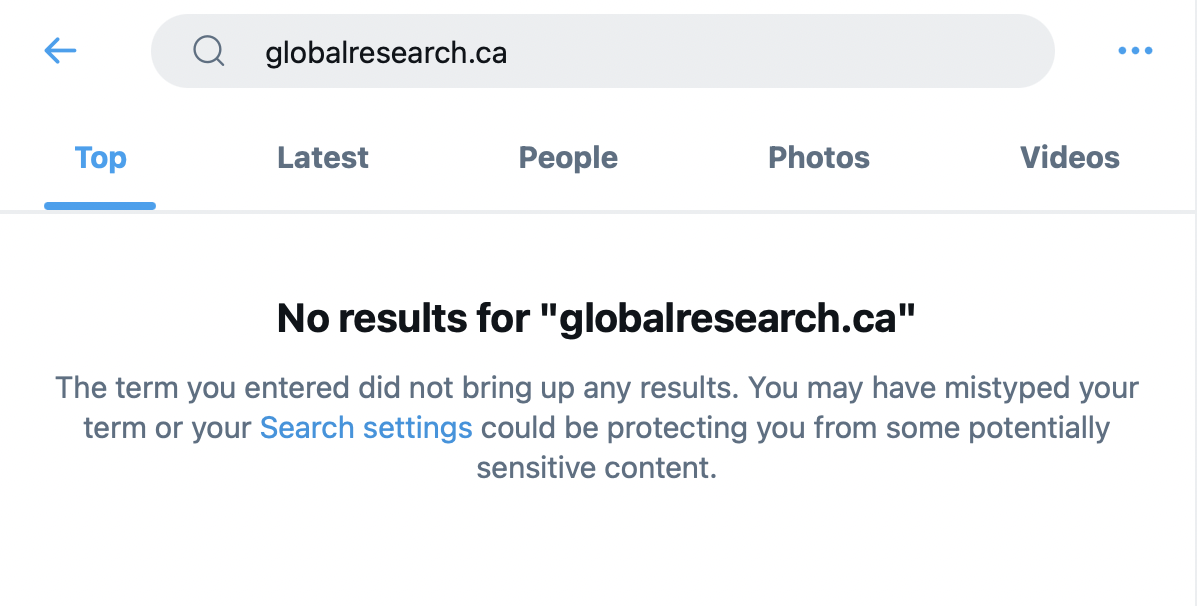
\includegraphics[scale=0.33]{./img/globalresearch_14_06_2021_16pm_UTC.png}\par
%\end{multicols}
%\caption{Screenshots taken on June 14, 2021. 
% }
%\label{fig3}
%\end{figure}

\begin{figure*}
\centering
\begin{multicols}{1}

    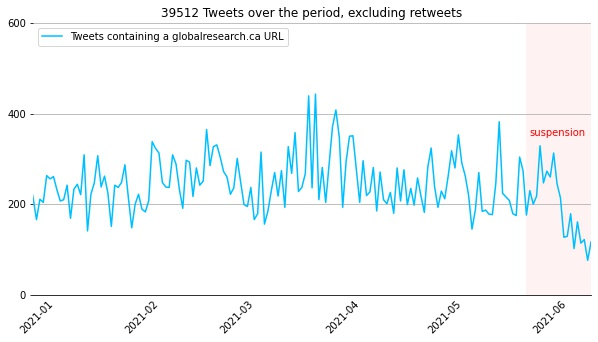
\includegraphics[scale=0.33]{./img/globalresearch/sum_globalresearch.ca_6_months.jpg}\par 
    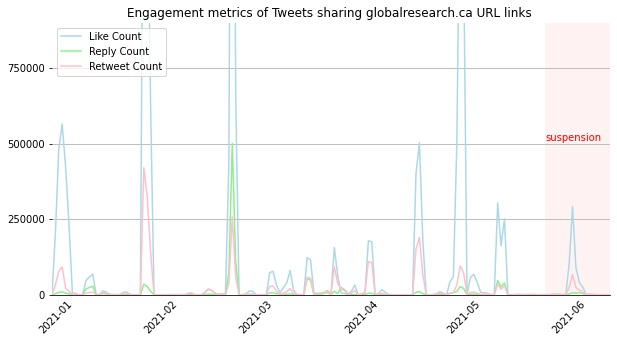
\includegraphics[scale=0.33]{./img/globalresearch/engagement_sum_rolling_1_globalresearch.ca.jpg}\par 
    \end{multicols}
\begin{multicols}{1}

  %  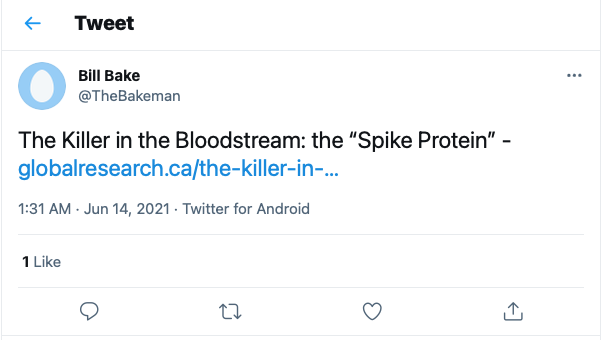
\includegraphics[scale=0.33]{./img/globalresearch/tweet.png}\par
    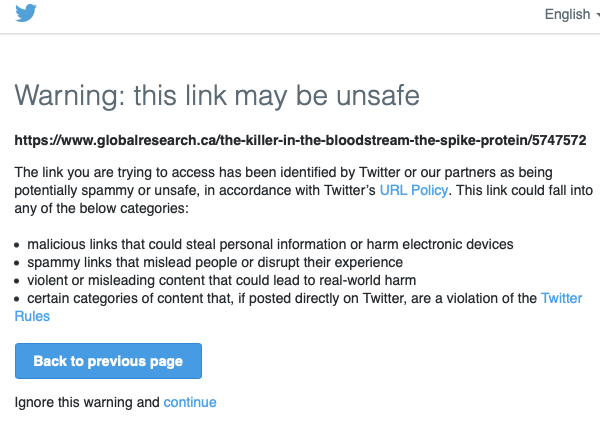
\includegraphics[scale=0.33]{./img/globalresearch/warning.png}\par
    \includegraphics[scale=0.33]{./img/globalresearch_14_06_2021_16pm_UTC.png}\par
\end{multicols}

%\begin{multicols}{1}
%
%  %  \includegraphics[scale=0.33]{./img/globalresearch_2021-06-14.png}\par
%    \includegraphics[scale=0.33]{./img/globalresearch_14_06_2021_16pm_UTC.png}\par
%\end{multicols}
\caption{ 
 }
\label{fig4}
\end{figure*}


%We provide a second example with the website $off$-$guardian.org$. Unlike the previous example, the Twitter account linked to this website is not currently\footnote{The account can be accessed via the Twitter handle $@OffGuardian0$ and we verified on June 13, 2021 that the account is not suspended.} suspended. 

%off guardian: people put space before .com but they can still share off-guardian links  (test Héloïse). why do they do that? 
%warning page before accessing the website - always 
%twitter API doesn't return the tweets tweeted by off-guardian themselves dating back to 2015
%twitter API returns both tweets with . org and .org: 320 tweets from 2017-01-15 until 2021-06-11. But off-guardian themselves posted one of their own links on June 16 2021. 
%minet returns almost nothing : 43 tweets 
% the tweets created by Off-Guardian: don't come up in the search box. Unlike nytimes.com their articles do appear in the search box , published by themselves! 
% Heloise's tweet June 15 doesn't come up in the API ! 
% people use variants with * and dot , so that they can find tweets speakign about those domains
\subsection{Flags and Notices}
\section{Discussion}

%→ Littérature liée aux effets psychologiques 
%→ multi-platforming, indirect effects, etc. 
%→ strategies 

\newpage 

\bibliography{proj1}{}
\bibliographystyle{plain}

\end{document}
